%initialising document, adjust papersize, fontsize and page orientation to your needs
\documentclass[a4paper, fontsize = 8pt, landscape]{scrartcl}
\usepackage{../../../misc_files/LateX/layout_and_colours}
\title{Software Entwicklung}
\author{Jil Zerndt, Lucien Perret}
\date{May 2024}

\createtitlepagestyle
\createmainpagestyle
\begin{document}
\begin{multicols}{3}
	\thispagestyle{TitlePageStyle}
	\maketitle
	\section{Einführung und Überblick}

\begin{definition}{Software Engineering}
\begin{itemize}
    \item Disziplinen: Anforderungen, Architektur, Implementierung, Test und Wartung.
    \item Ziel: Strukturierte Prozesse für Qualität, Risiko- und Fehlerminimierung.
\end{itemize}
\end{definition}

\begin{definition}{Modellierung in der Softwareentwicklung}
\begin{itemize}
    \item Modelle als Abstraktionen: Anforderungen, Architekturen, Testfälle.
    \item Einsatz von UML: Skizzen, detaillierte Blueprints, vollständige Spezifikationen.
    \end{itemize}
\end{definition}

\begin{concept}{Wrap-up}
\begin{itemize}
    \item Solide Analyse- und Entwurfskompetenzen sind essenziell.
    \item Iterativ-inkrementelle Modelle fördern agile Entwicklung.
\end{itemize}
\end{concept}

\subsection{Softwareentwicklungsprozesse}

\begin{concept}{Klassifizierung Software-Entwicklungs-Probleme}\\
  Wir betrachten Wasserfall, iterativ-inkrementelle und agile Softwareentwicklungsprozesse.\\
  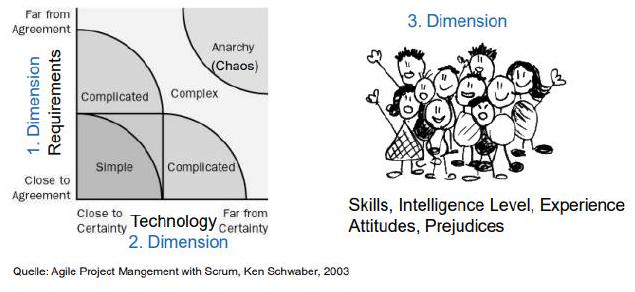
\includegraphics[width=\linewidth]{images/2024_12_29_0d1d7b5551ea1b4b41bdg-01}
\end{concept}


\begin{theorem}{Prozesse im Softwareengineering Kernprozesse}
\begin{itemize}
  \item Anforderungserhebung
  \item Systemdesign/technische Konzeption
  \item Implementierung
  \item Softwaretest
  \item Softwareeinführung
  \item Wartung/Pflege
\end{itemize}
\end{theorem}

\begin{corollary}{Unterstützungsprozesse}
\begin{itemize}
  \item Projektmanagement
  \item Qualitätsmanagement
  \item Risikomanagement
\end{itemize}
\end{corollary}

\begin{definition}{Begriffe}
  \begin{itemize}
    \item Warum wird modelliert: Um Analyse- und Designentwürfe zu diskutieren, abstimmen und zu dokumentieren bzw. zu kommunizieren.
    \item Modell: Ein Modell ist ein konkretes oder gedankliches Abbild eines vorhanden Gebildes oder Vorbild für ein zu schaffendes Gebilde (hier Softwareprodukt).
    \item Original: Das Original ist das abgebildete oder zu schaffende Gebilde.
    \item Modellierung: Modellierung gehört zum Fundament des Software Engineerings
  \end{itemize}
\end{definition}

\begin{concept}{Modelle in der Softwareentwicklung}
\begin{itemize}
  \item Software ist vielfach (immer?) selbst ein Modell
  \item Anforderungen sind Modelle der Problemstellung
  \item Architekturen und Entwürfe sind Modelle der Lösung
  \item Testfälle sind Modelle des korrekten Funktionierens des Codes usw.
\end{itemize}
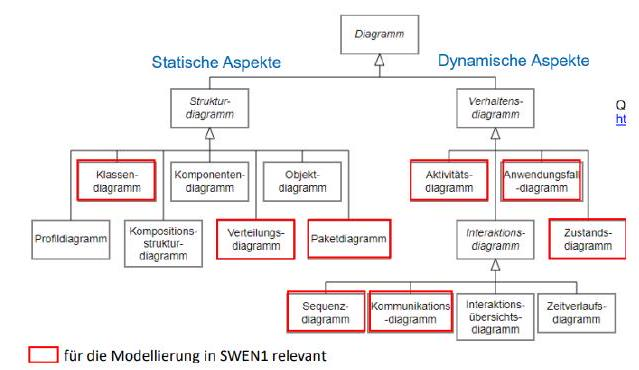
\includegraphics[width=\linewidth]{images/2024_12_29_0d1d7b5551ea1b4b41bdg-01(1)}
\end{concept}

\begin{definition}{Code and Fix}\\
Vorgehen, bei dem Codierung oder Korrektur im Wechsel mit Ad-hoc-Tests die einzigen bewussten ausgeführten Tätigkeiten der Software-Entwicklung sind: Schnell, Agil, Einfach am Anfang, Schlecht Planbar, Schlecht Wartbar, Änderungen s. Aufwändig
\end{definition}

\begin{definition}{Wasserfallmodell}\\
Die Software-Entwicklung wird als Folge von Aktivitäten/Phasen betrachtet, die durch Teilergebnisse (Dokumente) gekoppelt sind. Die Reihenfolge der Ak-\\
tivitäten ist fest definiert. : gut planbar, klare Aufteilung in Phasen, Schlechtes Risikomanagment, nie alle Anforderungen zu Anfang bekannt
\end{definition}

\begin{definition}{Iterativ-inkrementelle Modelle}\\
Software wird in mehreren geplanten und kontrolliert durchgeführten Iterationen schrittweise (inkrementell) entwickelt: Flexibles Modell, Gutes Risikomanagement, Frühe Einsetzbarkeit, Planung upfront hat Grenzen, Kunde Involviert über ganze Entwicklung\\
Agile Softwareentwicklung Basiert auf interativ-inkrementellen Prozessmodell, Fokussiert auf gut dokumentierten und getesteten Code statt auf ausführlicher Dokumentation
\end{definition}

\begin{concept}{Zweck und den Nutzen von Modellen in der Softwareentwicklung}\\
Modell von Requirements (close to/ far from Agreement) \& Technology (known / unknown)\\
Ein Modell ist ein konkretes oder gedankliches Abbild eines vorhanden Gebildes oder Vorbild für ein zu schaffendes Gebilde (hier Softwareprodukt).
\end{concept}

\begin{definition}{Unified Modelling Language (UML)}\\
UML ist die Standardsprache für die graphische Modellierung von Anforderungen, Analyse und Entwürfen im Software Engineering (objektorientierte Modellierung). (As a sketch, blueprint, programminglanguage)
\end{definition}

\begin{formula}{Incremental Model}\\
  Artefakte in einem iterativ-inkrementellen Prozess illustrieren und einordnen\\
\begin{center}
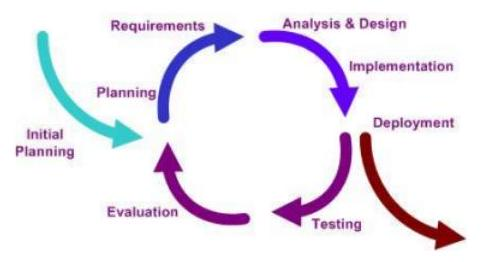
\includegraphics[width=0.8\linewidth]{images/2024_12_29_0d1d7b5551ea1b4b41bdg-02(1)}
\end{center}
\end{formula}
	\raggedcolumns
	\section{Anforderungsanalyse}

\subsubsection{Usability und User Experience}

\begin{concept}{Usability und User Experience}\\
Die drei Säulen der Benutzererfahrung:
\begin{itemize}
    \item \textbf{Usability (Gebrauchstauglichkeit):} Grundlegende Nutzbarkeit des Systems
    \item \textbf{User Experience:} Usability + Desirability (Attraktivität)
    \item \textbf{Customer Experience:} UX + Brand Experience (Markenwahrnehmung)
\end{itemize}
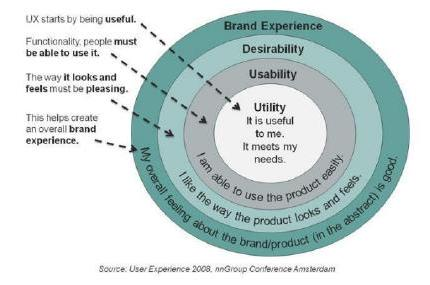
\includegraphics[width=0.9\linewidth]{images/2024_12_29_0d1d7b5551ea1b4b41bdg-02}
\end{concept}

\begin{definition}{Usability-Dimensionen}\\
Die drei Hauptdimensionen der Usability:
\begin{itemize}
    \item \textbf{Effektivität:}
    \begin{itemize}
        \item Vollständige Aufgabenerfüllung
        \item Gewünschte Genauigkeit
    \end{itemize}
    \item \textbf{Effizienz:} Minimaler Aufwand
    \begin{itemize}
        \item Mental
        \item Physisch
        \item Zeitlich
    \end{itemize}
    \item \textbf{Zufriedenheit:}
    \begin{itemize}
        \item Minimum: Keine Verärgerung
        \item Standard: Zufriedenheit
        \item Optimal: Begeisterung
    \end{itemize}
\end{itemize}
\end{definition}

\begin{theorem}{ISO 9241-110: Usability-Anforderungen}\\
Die sieben Grundprinzipien:
\begin{itemize}
    \item Aufgabenangemessenheit
    \item Lernförderlichkeit
    \item Individualisierbarkeit
    \item Erwartungskonformität
    \item Selbstbeschreibungsfähigkeit
    \item Steuerbarkeit
    \item Fehlertoleranz
\end{itemize}
\end{theorem}

\begin{concept}{User-Centered Design (UCD)}\\
Ein iterativer Prozess zur nutzerzentrierten Entwicklung:\\
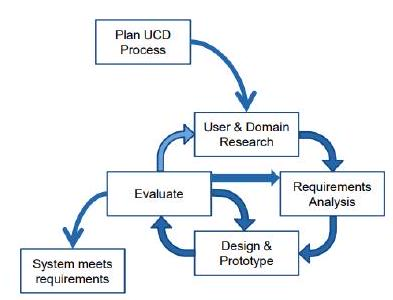
\includegraphics[width=0.6\linewidth]{images/2024_12_29_0d1d7b5551ea1b4b41bdg-03}
\end{concept}
\begin{theorem}{Wichtige Artefakte}
\begin{itemize}
    \item Personas: Repräsentative Nutzerprofile
    \item Usage-Szenarien: Konkrete Anwendungsfälle
    \item Mentales Modell: Nutzerverständnis
    \item Domänenmodell: Fachliches Verständnis
    \item Service Blueprint: Geschäftsprozessmodell
    \item Stakeholder Map: Beteiligte und Betroffene
    \item UI-Artefakte: Skizzen, Wireframes, Designs
\end{itemize}
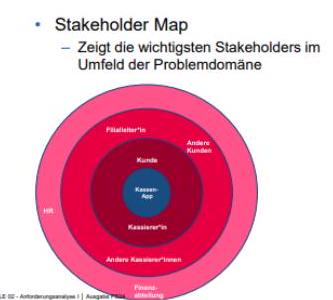
\includegraphics[width=0.5\linewidth]{images/2024_12_29_0d1d7b5551ea1b4b41bdg-04}
\end{theorem}

\subsubsection{Requirements Engineering}

\begin{definition}{Requirements (Anforderungen)}
\begin{itemize}
    \item Leistungsfähigkeiten oder Eigenschaften
    \item Explizit oder implizit
    \item Müssen mit allen Stakeholdern erarbeitet werden
    \item Entwickeln sich während des Projekts
\end{itemize}
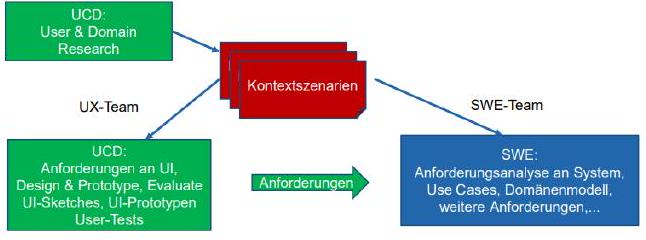
\includegraphics[width=\linewidth]{images/2024_12_29_0d1d7b5551ea1b4b41bdg-04(1)}
\end{definition}

\subsection{Use Cases}

\begin{definition}{Use Case (Anwendungsfall)}\\
Textuelle Beschreibung einer konkreten Interaktion zwischen Akteur und System:
\begin{itemize}
    \item Aus Sicht des Akteurs
    \item Aktiv formuliert
    \item Konkreter Nutzen
    \item Essentieller Stil (Logik statt Implementierung)
\end{itemize}
\end{definition}

\begin{theorem}{Akteure in Use Cases}
\begin{itemize}
    \item \textbf{Primärakteur:} Initiiert den Use Case, erhält Hauptnutzen
    \item \textbf{Unterstützender Akteur:} Hilft bei der Durchführung
    \item \textbf{Offstage-Akteur:} Indirekt beteiligter Stakeholder
\end{itemize}
\end{theorem}

\begin{KR}{Use Case Erstellung}\\
Schritte zur Erstellung eines vollständigen Use Cases:
\begin{enumerate}
    \item \textbf{Identifikation:}
    \begin{itemize}
        \item Systemgrenzen definieren
        \item Primärakteure identifizieren
        \item Ziele der Akteure ermitteln
    \end{itemize}
    \item \textbf{Dokumentation:}
    \begin{itemize}
        \item Brief/Casual für erste Analyse
        \item Fully-dressed für wichtige Use Cases
        \item Standardablauf und Erweiterungen
    \end{itemize}
    \item \textbf{Review:}
    \begin{itemize}
        \item Mit Stakeholdern abstimmen
        \item Auf Vollständigkeit prüfen
        \item Konsistenz sicherstellen
    \end{itemize}
\end{enumerate}
\end{KR}

\begin{example2}{Brief Use Case}
\textbf{Verkauf abwickeln}

Kunde kommt mit Waren zur Kasse. Kassier erfasst alle Produkte. System berechnet Gesamtbetrag. Kassier nimmt Zahlung entgegen und gibt ggf. Wechselgeld. System druckt Beleg.
\end{example2}

\begin{example2}{Fully-dressed Use Case}
\textbf{UC: Verkauf abwickeln}
\begin{itemize}
    \item \textbf{Umfang:} Kassensystem
    \item \textbf{Primärakteur:} Kassier
    \item \textbf{Stakeholder:} Kunde (schnelle Abwicklung), Geschäft (korrekte Abrechnung)
    \item \textbf{Vorbedingung:} Kasse ist geöffnet
    \item \textbf{Standardablauf:}
    \begin{enumerate}
        \item Kassier startet neuen Verkauf
        \item System initialisiert neue Transaktion
        \item Kassier erfasst Produkte
        \item System zeigt Zwischensumme
        \item Kassier schliesst Verkauf ab
        \item System zeigt Gesamtbetrag
        \item Kunde bezahlt
        \item System druckt Beleg
    \end{enumerate}
\end{itemize}
\end{example2}

\begin{concept}{Systemsequenzdiagramm (SSD)}\\
Formalisierte Darstellung der System-Interaktionen:
\begin{itemize}
    \item Zeigt Input/Output-Events
    \item Identifiziert Systemoperationen
    \item Basis für API-Design
\end{itemize}
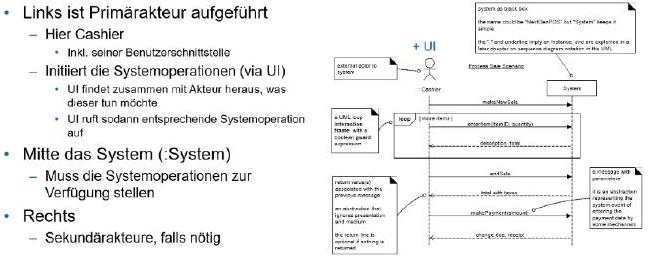
\includegraphics[width=\linewidth]{images/2024_12_29_0d1d7b5551ea1b4b41bdg-06}
\end{concept}

\begin{KR}{SSD Erstellung}
\begin{enumerate}
    \item Use Case als Grundlage wählen
    \item Akteur und System identifizieren
    \item Methodenaufrufe definieren:
    \begin{itemize}
        \item Namen aussagekräftig wählen
        \item Parameter festlegen
        \item Rückgabewerte bestimmen
    \end{itemize}
    \item Zeitliche Abfolge modellieren
    \item Optional: Externe Systeme einbinden
\end{enumerate}
\end{KR}

\begin{example}
\textbf{Aufgabe:} Erstellen Sie einen fully-dressed Use Case für ein Online-Bibliothekssystem. Fokus: "Buch ausleihen"

\textbf{Lösung:}
\begin{itemize}
    \item \textbf{Umfang:} Online-Bibliothekssystem
    \item \textbf{Primärakteur:} Bibliotheksnutzer
    \item \textbf{Stakeholder:} 
    \begin{itemize}
        \item Bibliotheksnutzer: Möchte Buch einfach ausleihen
        \item Bibliothek: Korrekte Erfassung der Ausleihe
    \end{itemize}
    \item \textbf{Vorbedingung:} Nutzer ist eingeloggt
    \item \textbf{Standardablauf:}
    \begin{enumerate}
        \item Nutzer sucht Buch
        \item System zeigt Verfügbarkeit
        \item Nutzer wählt Ausleihe
        \item System prüft Ausleihberechtigung
        \item System registriert Ausleihe
        \item System zeigt Bestätigung
    \end{enumerate}
    \item \textbf{Erweiterungen:}
    \begin{itemize}
        \item 2a: Buch nicht verfügbar
        \item 4a: Keine Ausleihberechtigung
    \end{itemize}
\end{itemize}
\end{example}

	\input{02_domänenmodellierung_new.tex}
	\section{Softwarearchitektur und Design}

\begin{concept}{Überblick Softwareentwicklung}\\
Die Entwicklung von Software erfolgt in verschiedenen Ebenen:
\begin{itemize}
    \item Business Analyse (Domänenmodell, Requirements)
    \item Architektur (Logische Struktur)
    \item Entwicklung (Konkrete Umsetzung)
\end{itemize}
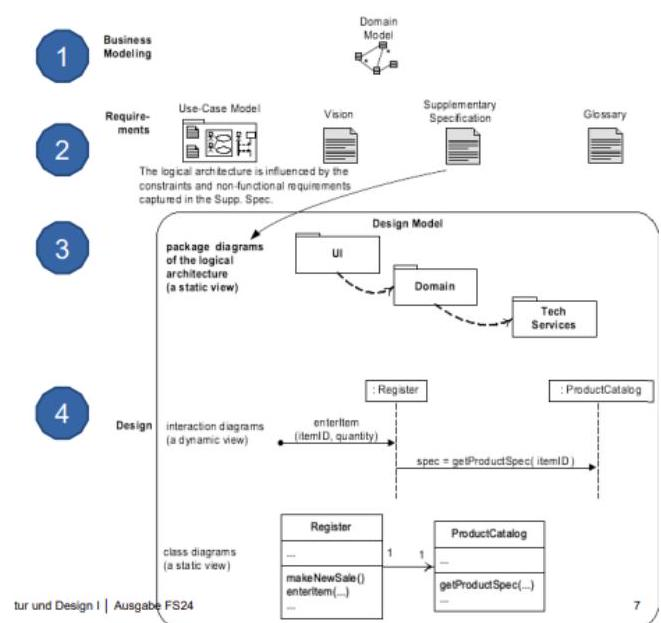
\includegraphics[width=0.9\linewidth]{images/2024_12_29_0d1d7b5551ea1b4b41bdg-07(2)}
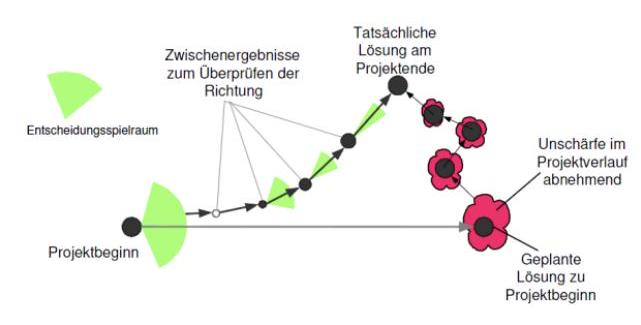
\includegraphics[width=0.9\linewidth]{images/2024_12_29_0d1d7b5551ea1b4b41bdg-08(1)}
\end{concept}

\begin{definition}{Softwarearchitektur}\\
Die Architektur definiert:
\begin{itemize}
    \item Grundlegende Strukturen und Komponenten
    \item Heutige und zukünftige Anforderungen
    \item Weiterentwicklungsmöglichkeiten
    \item Beziehungen zur Umgebung
\end{itemize}
\end{definition}

\begin{concept}{Architekturanalyse}\\
Die Analyse erfolgt iterativ mit den Anforderungen:
\begin{itemize}
    \item Analyse funktionaler und nicht-funktionaler Anforderungen
    \item Abstimmung mit Stakeholdern
    \item Kontinuierliche Weiterentwicklung
\end{itemize}
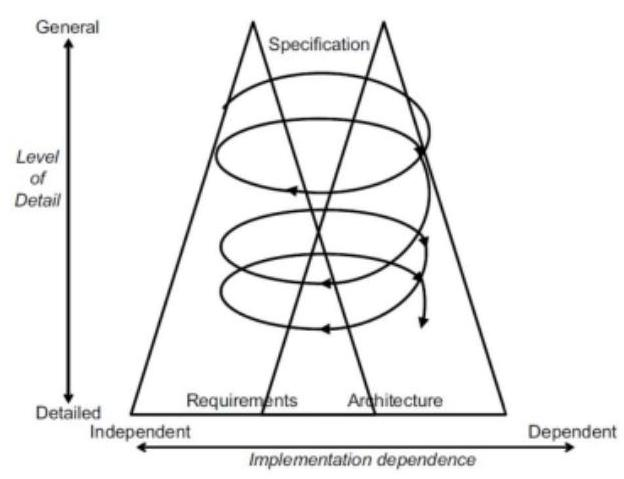
\includegraphics[width=0.9\linewidth]{images/2024_12_29_0d1d7b5551ea1b4b41bdg-08}
\end{concept}

\begin{theorem}{ISO 25010 vs FURPS+}\\
\textbf{ISO 25010:}
\begin{itemize}
    \item Hierarchische Struktur für nicht-funktionale Anforderungen
    \item Definierte Hauptcharakteristiken und Subcharakteristiken
    \item Messbare Metriken für jede Anforderung
    \item Präzise Formulierung und Verifikation
\end{itemize}

\textbf{FURPS+:}
\begin{itemize}
    \item Functionality (Funktionalität)
    \item Usability (Benutzbarkeit)
    \item Reliability (Zuverlässigkeit)
    \item Performance (Leistung)
    \item Supportability (Wartbarkeit)
    \item + (Implementation, Interface, Operations, Packaging, Legal)
\end{itemize}
\end{theorem}

\begin{concept}{Modulkonzept}\\
Ein Modul (Baustein, Komponente) wird bewertet nach:
\begin{itemize}
    \item \textbf{Kohäsion:} Innerer Zusammenhang
    \item \textbf{Kopplung:} Externe Abhängigkeiten
\end{itemize}

\textbf{Eigenschaften:}
\begin{itemize}
    \item Autarkes Teilsystem
    \item Minimale externe Schnittstellen
    \item Enthält alle benötigten Funktionen/Daten
    \item Verschiedene Formen: Paket, Library, Service
\end{itemize}
\end{concept}

\begin{concept}{Architektursichten}\\
Das N+1 View Model beschreibt verschiedene Perspektiven:
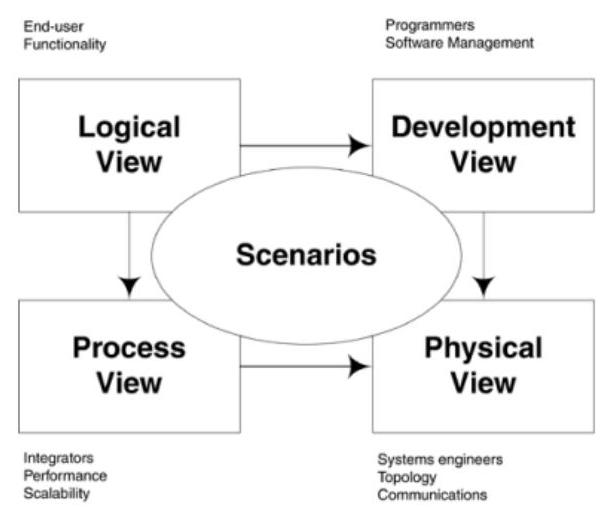
\includegraphics[width=0.9\linewidth]{images/2024_12_29_0d1d7b5551ea1b4b41bdg-09}

\textbf{UML-Paketdiagramm:}
\begin{itemize}
    \item Definition von Teilsystemen
    \item Gruppierung von Elementen
    \item Abhängigkeiten zwischen Paketen
\end{itemize}
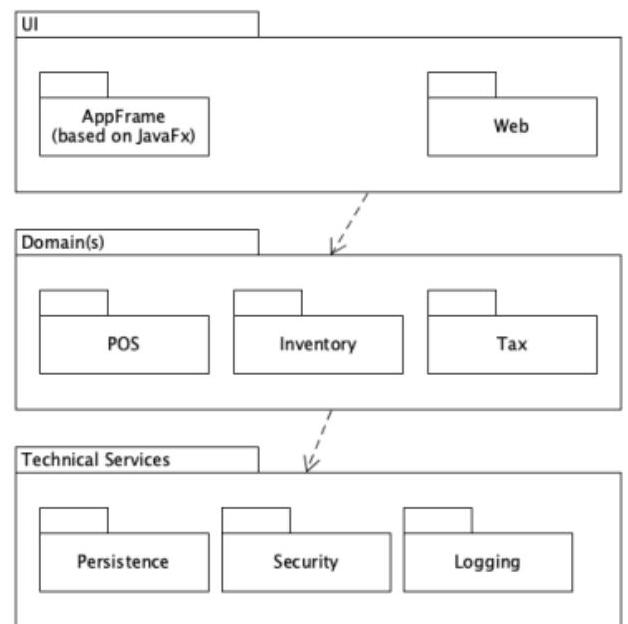
\includegraphics[width=0.9\linewidth]{images/2024_12_29_0d1d7b5551ea1b4b41bdg-09(1)}
\end{concept}

\subsubsection{UML-Modellierung}

\begin{KR}{Statische vs. Dynamische Modelle}\\
\textbf{Statische Modelle (Struktur):}
\begin{itemize}
    \item UML-Klassendiagramm
    \item Fokus auf Pakete, Klassen, Attribute
    \item Keine Methodenimplementierung
\end{itemize}

\textbf{Dynamische Modelle (Verhalten):}
\begin{itemize}
    \item UML-Interaktionsdiagramme
    \item Fokus auf Logik und Verhalten
    \item Implementierung der Methoden
\end{itemize}
\end{KR}

\begin{definition}{UML-Diagrammtypen}\\
\textbf{1. Klassendiagramm:}
\begin{itemize}
    \item Klassen und aktive Klassen
    \item Attribute und Operationen
    \item Sichtbarkeiten und Beziehungen
    \item Interfaces und Realisierungen
\end{itemize}

\textbf{2. Sequenzdiagramm:}
\begin{itemize}
    \item Lebenslinien und Nachrichten
    \item Synchrone/Asynchrone Kommunikation
    \item Aktivierung und Deaktivierung
    \item Alternative Abläufe
\end{itemize}

\textbf{3. Zustandsdiagramm:}
\begin{itemize}
    \item Zustände und Übergänge
    \item Start- und Endzustände
    \item Composite States
    \item Historie und Parallelität
\end{itemize}

\textbf{4. Aktivitätsdiagramm:}
\begin{itemize}
    \item Aktionen und Aktivitäten
    \item Kontroll- und Datenflüsse
    \item Verzweigungen und Zusammenführungen
    \item Partitionen (Swimlanes)
\end{itemize}
\end{definition}

\begin{concept}{Responsibility Driven Design (RDD)}\\
Design basierend auf Verantwortlichkeiten:
\begin{itemize}
    \item Klassenentwurf nach Rollen
    \item Kollaborationsbeziehungen
    \item Implementierung durch Attribute/Methoden
    \item Anwendbar auf allen Ebenen
\end{itemize}
\end{concept}

\begin{theorem}{GRASP Prinzipien}\\
General Responsibility Assignment Software Patterns:
\begin{itemize}
    \item \textbf{Information Expert:} Verantwortung basierend auf Information
    \item \textbf{Creator:} Objekterstellung bei starker Beziehung
    \item \textbf{Controller:} Zentrale Steuerungslogik
    \item \textbf{Low Coupling:} Minimale Abhängigkeiten
    \item \textbf{High Cohesion:} Starker innerer Zusammenhang
    \item \textbf{Polymorphism:} Flexibilität durch Schnittstellen
    \item \textbf{Pure Fabrication:} Künstliche Klassen für besseres Design
    \item \textbf{Indirection:} Vermittler für Flexibilität
    \item \textbf{Protected Variations:} Kapselung von Änderungen
\end{itemize}
\end{theorem}

\begin{example}{Architekturentwurf}
\textbf{Aufgabe:} Entwerfen Sie die grundlegende Architektur für ein Online-Banking-System.

\textbf{Lösung:}
\begin{itemize}
    \item \textbf{Anforderungsanalyse:}
    \begin{itemize}
        \item Sicherheit (ISO 25010)
        \item Performance (FURPS+)
        \item Skalierbarkeit
    \end{itemize}
    
    \item \textbf{Architekturentscheidungen:}
    \begin{itemize}
        \item Mehrschichtige Architektur
        \item Microservices für Skalierbarkeit
        \item Sicherheitsschicht
    \end{itemize}
    
    \item \textbf{Module:}
    \begin{itemize}
        \item Authentifizierung
        \item Transaktionen
        \item Kontoführung
    \end{itemize}
\end{itemize}
\end{example}

\begin{KR}{Architekturentwurf}
\textbf{Schritte:}
\begin{enumerate}
    \item Anforderungen analysieren
    \item Architekturstil wählen
    \item Module identifizieren
    \item Schnittstellen definieren
    \item Mit Stakeholdern abstimmen
\end{enumerate}

\textbf{Qualitätskriterien:}
\begin{itemize}
    \item Änderbarkeit
    \item Wartbarkeit
    \item Erweiterbarkeit
    \item Testbarkeit
\end{itemize}
\end{KR}
	\section{Use Case Realisation}

\begin{concept}{Use Case Realization}\\
Die Umsetzung von Use Cases erfolgt durch:
\begin{itemize}
    \item Detaillierte Szenarien aus den Use Cases
    \item Systemantworten müssen realisiert werden
    \item UI statt System im SSD
    \item Systemoperationen sind die zu implementierenden Elemente
\end{itemize}
\end{concept}

\begin{definition}{UML im Implementierungsprozess}\\
UML dient als:
\begin{itemize}
    \item Zwischenschritt bei wenig Erfahrung
    \item Kompakter Ersatz für Programmiercode
    \item Kommunikationsmittel (auch für Nicht-Techniker)
\end{itemize}
\end{definition}

\begin{KR}{Vorgehen bei der Use Case Realization}\\
\textbf{1. Vorbereitung:}
\begin{itemize}
    \item Use Case auswählen und SSD ableiten
    \item Systemoperation identifizieren
    \item Operation Contract erstellen/prüfen
\end{itemize}

\textbf{2. Analyse:}
\begin{itemize}
    \item Aktuellen Code/Dokumentation analysieren
    \item DCD überprüfen/aktualisieren
    \item Vergleich mit Domänenmodell
    \item Neue Klassen gemäß Domänenmodell erstellen
\end{itemize}

\textbf{3. Realisierung:}
\begin{itemize}
    \item Controller Klasse bestimmen
    \item Zu verändernde Klassen festlegen
    \item Weg zu diesen Klassen festlegen:
    \begin{itemize}
        \item Parameter für Wege definieren
        \item Klassen bei Bedarf erstellen
        \item Verantwortlichkeiten zuweisen
        \item Verschiedene Varianten evaluieren
    \end{itemize}
    \item Veränderungen implementieren
    \item Review durchführen
\end{itemize}
\end{KR}

\begin{example}{Use Case Realization: Verkauf abwickeln}
\textbf{1. Vorbereitung:}
\begin{itemize}
    \item \textbf{Use Case:} Verkauf abwickeln
    \item \textbf{Systemoperation:} makeNewSale()
    \item \textbf{Contract:} Neue Sale-Instanz wird erstellt
\end{itemize}

\textbf{2. Analyse:}
\begin{itemize}
    \item \textbf{Klassen:} Register, Sale
    \item \textbf{DCD:} Beziehung Register-Sale prüfen
    \item \textbf{Neue Klassen:} Payment, SaleLineItem
\end{itemize}

\textbf{3. Implementierung:}
\begin{itemize}
    \item Register als Controller
    \item Sale-Klasse erweitern
    \item Beziehungen implementieren
\end{itemize}
\end{example}

\begin{KR}{Typische Implementierungsfehler vermeiden}\\
\begin{itemize}
    \item \textbf{Architekturverletzungen:}
    \begin{itemize}
        \item Schichtentrennung beachten
        \item Abhängigkeiten richtig setzen
    \end{itemize}
    
    \item \textbf{GRASP-Verletzungen:}
    \begin{itemize}
        \item Information Expert beachten
        \item Creator Pattern richtig anwenden
        \item High Cohesion erhalten
    \end{itemize}
    
    \item \textbf{Testbarkeit:}
    \begin{itemize}
        \item Klassen isoliert testbar halten
        \item Abhängigkeiten mockbar gestalten
    \end{itemize}
\end{itemize}
\end{KR}

	\section{Design Patterns}

\begin{concept}{Grundlagen Design Patterns}\\
Bewährte Lösungsmuster für wiederkehrende Probleme:
\begin{itemize}
    \item Beschleunigen Entwicklung durch vorgefertigte Lösungen
    \item Verbessern Kommunikation im Team
    \item Bieten Balance zwischen Flexibilität und Komplexität
    \item \textbf{Wichtig:} Design Patterns sind kein Selbstzweck
\end{itemize}
\end{concept}

\subsection{Grundlegende Design Patterns}

\begin{definition}{Adapter Pattern}\\
\textbf{Problem:} Inkompatible Schnittstellen
\begin{itemize}
    \item Objekte mit unterschiedlichen Interfaces sollen zusammenarbeiten
    \item Externe Dienste sollen austauschbar sein
\end{itemize}
\textbf{Lösung:} Adapter-Klasse als Vermittler
\end{definition}

\begin{definition}{Simple Factory Pattern}\\
\textbf{Problem:} Komplexe Objekterzeugung
\begin{itemize}
    \item Objekterzeugung erfordert viele Schritte
    \item Konfiguration bei Erzeugung notwendig
\end{itemize}
\textbf{Lösung:} Eigene Klasse für Objekterzeugung
\end{definition}

\begin{definition}{Singleton Pattern}\\
\textbf{Problem:} Genau eine Instanz benötigt
\begin{itemize}
    \item Globaler Zugriffspunkt notwendig
    \item Mehrfachinstanzierung verhindern
\end{itemize}
\textbf{Lösung:} Statische Instanz mit privater Erzeugung
\end{definition}

\begin{definition}{Dependency Injection Pattern}\\
\textbf{Problem:} Abhängigkeiten zu anderen Objekten
\begin{itemize}
    \item Lose Kopplung erwünscht
    \item Flexibilität bei Abhängigkeiten
\end{itemize}
\textbf{Lösung:} Abhängigkeiten werden von außen injiziert
\end{definition}

\begin{definition}{Proxy Pattern}\\
\textbf{Problem:} Zugriffskontrolle auf Objekte
\begin{itemize}
    \item Verzögertes Laden
    \item Zugriffsbeschränkungen
    \item Netzwerkkommunikation
\end{itemize}
\textbf{Lösung:} Stellvertreterobjekt mit gleichem Interface
\begin{itemize}
    \item \textbf{Remote Proxy:} Für entfernte Objekte
    \item \textbf{Virtual Proxy:} Für spätes Laden
    \item \textbf{Protection Proxy:} Für Zugriffsschutz
\end{itemize}
\end{definition}

\begin{definition}{Chain of Responsibility Pattern}\\
\textbf{Problem:} Unklare Zuständigkeit für Anfragen
\begin{itemize}
    \item Mehrere mögliche Handler
    \item Zuständigkeit erst zur Laufzeit klar
\end{itemize}
\textbf{Lösung:} Verkettete Handler-Objekte
\end{definition}

\subsection{Erweiterte Design Patterns}

\begin{definition}{Decorator Pattern}\\
\textbf{Problem:} Dynamische Erweiterung von Objekten
\begin{itemize}
    \item Zusätzliche Verantwortlichkeiten
    \item Nur für einzelne Objekte
\end{itemize}
\textbf{Lösung:} Wrapper-Objekt mit gleichem Interface
\end{definition}

\begin{definition}{Observer Pattern}\\
\textbf{Problem:} Abhängige Objekte aktualisieren
\begin{itemize}
    \item Lose Kopplung erwünscht
    \item Typ des Empfängers unbekannt
\end{itemize}
\textbf{Lösung:} Observer-Interface für Benachrichtigungen
\end{definition}

\begin{definition}{Strategy Pattern}\\
\textbf{Problem:} Austauschbare Algorithmen
\begin{itemize}
    \item Verschiedene Implementierungen
    \item Zur Laufzeit wechselbar
\end{itemize}
\textbf{Lösung:} Interface für Algorithmus-Klassen
\end{definition}

\begin{definition}{Composite Pattern}\\
\textbf{Problem:} Baumstrukturen verwalten
\begin{itemize}
    \item Einheitliche Behandlung
    \item Teil-Ganzes Hierarchie
\end{itemize}
\textbf{Lösung:} Gemeinsames Interface für Container und Inhalt
\end{definition}

\begin{KR}{Design Pattern Auswahl}\\
\textbf{Schritt 1: Problem analysieren}
\begin{itemize}
    \item Art des Problems identifizieren
    \item Anforderungen klar definieren
    \item Kontext verstehen
\end{itemize}

\textbf{Schritt 2: Pattern evaluieren}
\begin{itemize}
    \item Passende Patterns suchen
    \item Vor- und Nachteile abwägen
    \item Komplexität bewerten
\end{itemize}

\textbf{Schritt 3: Implementation planen}
\begin{itemize}
    \item Klassenstruktur entwerfen
    \item Schnittstellen definieren
    \item Anpassungen vornehmen
\end{itemize}
\end{KR}



	\begin{example}{Adapter Pattern}\\
\textbf{Szenario:} Altbestand an Drittanbieter-Bibliothek integrieren
\begin{lstlisting}[language=Java, style=base] 
// Bestehende Schnittstelle
interface ModernPrinter {
    void printDocument(String content);
}

// Alte Drittanbieter-Klasse
class LegacyPrinter {
    public void print(String[] pages) {
        for(String page : pages) {
            System.out.println(page);
        }
    }
}

// Adapter
class PrinterAdapter implements ModernPrinter {
    private LegacyPrinter legacyPrinter;
    
    public PrinterAdapter(LegacyPrinter printer) {
        this.legacyPrinter = printer;
    }
    
    public void printDocument(String content) {
        String[] pages = content.split("\n");
        legacyPrinter.print(pages);
    }
}
\end{lstlisting}
\end{example}

\begin{example}{Simple Factory}\\
\textbf{Szenario:} Erzeugung von verschiedenen Datenbankverbindungen
\begin{lstlisting}[language=Java, style=base]
class DatabaseFactory {
    public static Database createDatabase(String type) {
        switch(type) {
            case "MySQL":
                return new MySQLDatabase();
            case "PostgreSQL":
                return new PostgreSQLDatabase();
            default:
                throw new IllegalArgumentException("Unknown DB type");
        }
    }
}

// Verwendung
Database db = DatabaseFactory.createDatabase("MySQL");
\end{lstlisting}
\end{example}

\begin{example}{Singleton}\\
\textbf{Szenario:} Globale Konfigurationsverwaltung
\begin{lstlisting}[language=Java, style=base]
public class Configuration {
    private static Configuration instance;
    private Map<String, String> config;
    
    private Configuration() {
        config = new HashMap<>();
    }
    
    public static Configuration getInstance() {
        if(instance == null) {
            instance = new Configuration();
        }
        return instance;
    }
}
\end{lstlisting}
\end{example}

\begin{example}{Dependency Injection}\\
\textbf{Szenario:} Flexible Logger-Implementation
\begin{lstlisting}[language=Java, style=base]
interface Logger {
    void log(String message);
}

class FileLogger implements Logger {
    public void log(String message) {
        // Log to file
    }
}

class UserService {
    private final Logger logger;
    
    public UserService(Logger logger) { // Dependency Injection
        this.logger = logger;
    }
}
\end{lstlisting}
\end{example}

\begin{example}{Proxy}\\
\textbf{Szenario:} Verzögertes Laden eines großen Bildes
\begin{lstlisting}[language=Java, style=base]
interface Image {
    void display();
}

class RealImage implements Image {
    private String filename;
    
    public RealImage(String filename) {
        this.filename = filename;
        loadFromDisk();
    }
    
    private void loadFromDisk() {
        System.out.println("Loading " + filename);
    }
    
    public void display() {
        System.out.println("Displaying " + filename);
    }
}

class ImageProxy implements Image {
    private RealImage realImage;
    private String filename;
    
    public ImageProxy(String filename) {
        this.filename = filename;
    }
    
    public void display() {
        if(realImage == null) {
            realImage = new RealImage(filename);
        }
        realImage.display();
    }
}
\end{lstlisting}
\end{example}

\begin{example}{Chain of Responsibility}\\
\textbf{Szenario:} Authentifizierungskette
\begin{lstlisting}[language=Java, style=base]
abstract class AuthHandler {
    protected AuthHandler next;
    
    public void setNext(AuthHandler next) {
        this.next = next;
    }
    
    public abstract boolean handle(String username, String password);
}

class LocalAuthHandler extends AuthHandler {
    public boolean handle(String username, String password) {
        if(checkLocalDB(username, password)) {
            return true;
        }
        return next != null ? next.handle(username, password) : false;
    }
}

class LDAPAuthHandler extends AuthHandler {
    public boolean handle(String username, String password) {
        if(checkLDAP(username, password)) {
            return true;
        }
        return next != null ? next.handle(username, password) : false;
    }
}
\end{lstlisting}
\end{example}

\begin{example}{Decorator}\\
\textbf{Szenario:} Dynamische Erweiterung eines Text-Editors
\begin{lstlisting}[language=Java, style=base]
interface TextComponent {
    String render();
}

class SimpleText implements TextComponent {
    private String text;
    
    public SimpleText(String text) {
        this.text = text;
    }
    
    public String render() {
        return text;
    }
}

class BoldDecorator implements TextComponent {
    private TextComponent component;
    
    public BoldDecorator(TextComponent component) {
        this.component = component;
    }
    
    public String render() {
        return "<b>" + component.render() + "</b>";
    }
}
\end{lstlisting}
\end{example}

\begin{example}{Observer}\\
\textbf{Szenario:} News-Benachrichtigungssystem
\begin{lstlisting}[language=Java, style=base]
interface NewsObserver {
    void update(String news);
}

class NewsAgency {
    private List<NewsObserver> observers = new ArrayList<>();
    
    public void addObserver(NewsObserver observer) {
        observers.add(observer);
    }
    
    public void notifyObservers(String news) {
        for(NewsObserver observer : observers) {
            observer.update(news);
        }
    }
}

class NewsChannel implements NewsObserver {
    private String name;
    
    public NewsChannel(String name) {
        this.name = name;
    }
    
    public void update(String news) {
        System.out.println(name + " received: " + news);
    }
}
\end{lstlisting}
\end{example}

\begin{example}{Strategy}\\
\textbf{Szenario:} Verschiedene Zahlungsmethoden
\begin{lstlisting}[language=Java, style=base]
interface PaymentStrategy {
    void pay(int amount);
}

class CreditCardPayment implements PaymentStrategy {
    private String cardNumber;
    
    public void pay(int amount) {
        System.out.println("Paid " + amount + " using Credit Card");
    }
}

class PayPalPayment implements PaymentStrategy {
    private String email;
    
    public void pay(int amount) {
        System.out.println("Paid " + amount + " using PayPal");
    }
}
\end{lstlisting}
\end{example}

\begin{example}{Composite}\\
\textbf{Szenario:} Dateisystem-Struktur
\begin{lstlisting}[language=Java, style=base]
interface FileSystemComponent {
    void list(String prefix);
}

class File implements FileSystemComponent {
    private String name;
    
    public void list(String prefix) {
        System.out.println(prefix + name);
    }
}

class Directory implements FileSystemComponent {
    private String name;
    private List<FileSystemComponent> children = new ArrayList<>();
    
    public void add(FileSystemComponent component) {
        children.add(component);
    }
    
    public void list(String prefix) {
        System.out.println(prefix + name);
        for(FileSystemComponent child : children) {
            child.list(prefix + "  ");
        }
    }
}
\end{lstlisting}
\end{example}

\begin{example}{State}\\
\textbf{Szenario:} Verkaufsautomat
\begin{lstlisting}[language=Java, style=base]
interface VendingMachineState {
    void insertCoin();
    void ejectCoin();
    void selectProduct();
    void dispense();
}

class HasCoinState implements VendingMachineState {
    private VendingMachine machine;
    
    public void selectProduct() {
        System.out.println("Product selected");
        machine.setState(machine.getSoldState());
    }
    
    public void insertCoin() {
        System.out.println("Already have coin");
    }
}

class VendingMachine {
    private VendingMachineState currentState;
    
    public void setState(VendingMachineState state) {
        this.currentState = state;
    }
    
    public void insertCoin() {
        currentState.insertCoin();
    }
}
\end{lstlisting}
\end{example}

\begin{example}{Visitor}\\
\textbf{Szenario:} Dokumentstruktur mit verschiedenen Operationen
\begin{lstlisting}[language=Java, style=base]
interface DocumentElement {
    void accept(Visitor visitor);
}

interface Visitor {
    void visit(Paragraph paragraph);
    void visit(Heading heading);
}

class HTMLVisitor implements Visitor {
    public void visit(Paragraph p) {
        System.out.println("<p>" + p.getText() + "</p>");
    }
    
    public void visit(Heading h) {
        System.out.println("<h1>" + h.getText() + "</h1>");
    }
}
\end{lstlisting}
\end{example}

\begin{example}{Facade}\\
\textbf{Szenario:} Vereinfachte Multimedia-Bibliothek
\begin{lstlisting}[language=Java, style=base]
class MultimediaFacade {
    private AudioSystem audio;
    private VideoSystem video;
    private SubtitleSystem subtitles;
    
    public void playMovie(String movie) {
        audio.initialize();
        video.initialize();
        subtitles.load(movie);
        video.play(movie);
        audio.play();
    }
}
\end{lstlisting}
\end{example}

\begin{example}{Abstract Factory}\\
\textbf{Szenario:} GUI-Elemente für verschiedene Betriebssysteme
\begin{lstlisting}[language=Java, style=base]
interface GUIFactory {
    Button createButton();
    Checkbox createCheckbox();
}

class WindowsFactory implements GUIFactory {
    public Button createButton() {
        return new WindowsButton();
    }
    
    public Checkbox createCheckbox() {
        return new WindowsCheckbox();
    }
}

class MacFactory implements GUIFactory {
    public Button createButton() {
        return new MacButton();
    }
    
    public Checkbox createCheckbox() {
        return new MacCheckbox();
    }
}
\end{lstlisting}
\end{example}

\begin{example}{Factory Method Implementation}\\
\textbf{Aufgabe:} Implementieren Sie eine Factory für verschiedene Dokumenttypen (PDF, Word, Text)

\textbf{Lösung:}
\begin{lstlisting}[language=Java, style=base]
// Interface fuer Produkte
interface Document {
    void open();
    void save();
}

// Konkrete Produkte
class PdfDocument implements Document {
    public void open() { /* ... */ }
    public void save() { /* ... */ }
}

// Factory Method Pattern
abstract class DocumentCreator {
    abstract Document createDocument();
    
    // Template Method
    final void processDocument() {
        Document doc = createDocument();
        doc.open();
        doc.save();
    }
}

// Konkrete Factory
class PdfDocumentCreator extends DocumentCreator {
    Document createDocument() {
        return new PdfDocument();
    }
}
\end{lstlisting}
\end{example}

\begin{example}{Observer Pattern Implementation}\\
\textbf{Aufgabe:} Implementieren Sie ein Benachrichtigungssystem für Aktienkurse

\textbf{Lösung:}
\begin{lstlisting}[language=Java, style=base]
interface StockObserver {
    void update(String stock, double price);
}

class StockMarket {
    private List<StockObserver> observers = new ArrayList<>();
    
    public void attach(StockObserver observer) {
        observers.add(observer);
    }
    
    public void notifyObservers(String stock, double price) {
        for(StockObserver observer : observers) {
            observer.update(stock, price);
        }
    }
}

class StockDisplay implements StockObserver {
    public void update(String stock, double price) {
        System.out.println("Stock: " + stock + 
                         " updated to " + price);
    }
}
\end{lstlisting}
\end{example}
	\raggedcolumns
	\section{Implementation, Refactoring und Testing}

\subsection{Von Design zu Code}

\begin{concept}{Implementierungsstrategien}\\
\textbf{1. Bottom-Up Entwicklung:}
\begin{itemize}
    \item Implementierung beginnt mit Basisbausteinen
    \item Schrittweise Integration zu größeren Komponenten
    \item \textbf{Vorteile:} Gründlich, solide Basis
    \item \textbf{Nachteile:} Spätes Feedback
\end{itemize}

\textbf{2. Agile Entwicklung:}
\begin{itemize}
    \item Inkrementelle Entwicklung in Sprints
    \item Kontinuierliche Integration und Auslieferung
    \item \textbf{Vorteile:} Flexibilität, schnelles Feedback
    \item \textbf{Nachteile:} Mögliche Restrukturierung nötig
\end{itemize}
\end{concept}

\begin{definition}{Entwicklungsansätze}\\
\textbf{Code-Driven Development (CDD):}
\begin{itemize}
    \item Direkte Implementierung der Klassen
    \item Nachträgliches Testing
\end{itemize}

\textbf{Test-Driven Development (TDD):}
\begin{itemize}
    \item Tests vor Implementation
    \item Red-Green-Refactor Zyklus
\end{itemize}

\textbf{Behavior-Driven Development (BDD):}
\begin{itemize}
    \item Testbeschreibung aus Anwendersicht
    \item Gherkin-Syntax für Szenarios
\end{itemize}
\end{definition}

\begin{KR}{Clean Code}\\
\textbf{1. Code-Guidelines:}
\begin{itemize}
    \item Einheitliche Formatierung
    \item Klare Namenskonventionen
    \item Dokumentationsrichtlinien
\end{itemize}

\textbf{2. Fehlerbehandlung:}
\begin{itemize}
    \item Exceptions statt Fehlercodes
    \item Sinnvolle Error Messages
    \item Logging-Strategie
\end{itemize}

\textbf{3. Namensgebung:}
\begin{itemize}
    \item Aussagekräftige Namen
    \item Konsistente Begriffe
    \item Domain-Driven Naming
\end{itemize}
\end{KR}

\begin{concept}{Laufzeit-Optimierung}\\
\textbf{Grundregeln:}
\begin{itemize}
    \item Zuerst messen, dann optimieren
    \item Performance-Profile nutzen
    \item Bottlenecks identifizieren
\end{itemize}

\textbf{Häufige Probleme:}
\begin{itemize}
    \item Datenbank-Zugriffe
    \item Ineffiziente Algorithmen
    \item Speicherlecks
\end{itemize}
\end{concept}

\subsection{Refactoring}

\begin{definition}{Refactoring Grundlagen}\\
Strukturierte Verbesserung des Codes ohne Änderung des externen Verhaltens:
\begin{itemize}
    \item Kleine, kontrollierte Schritte
    \item Erhaltung der Funktionalität
    \item Verbesserung der Codequalität
\end{itemize}
\end{definition}

\begin{KR}{Refactoring Durchführung}\\
\textbf{1. Code Smells identifizieren:}
\begin{itemize}
    \item Duplizierter Code
    \item Lange Methoden
    \item Große Klassen
    \item Hohe Kopplung
\end{itemize}

\textbf{2. Refactoring durchführen:}
\begin{itemize}
    \item Tests sicherstellen
    \item Änderungen vornehmen
    \item Tests ausführen
\end{itemize}

\textbf{3. Patterns anwenden:}
\begin{itemize}
    \item Extract Method
    \item Move Method
    \item Rename
    \item Introduce Variable
\end{itemize}
\end{KR}



\subsection{Testing}

\begin{definition}{Testarten}\\
\textbf{Nach Sicht:}
\begin{itemize}
    \item \textbf{Black-Box:} Funktionaler Test ohne Codekenntnis
    \item \textbf{White-Box:} Strukturbezogener Test mit Codekenntnis
\end{itemize}

\textbf{Nach Umfang:}
\begin{itemize}
    \item \textbf{Unit-Tests:} Einzelne Komponenten
    \item \textbf{Integrationstests:} Zusammenspiel
    \item \textbf{Systemtests:} Gesamtsystem
    \item \textbf{Akzeptanztests:} Kundenanforderungen
\end{itemize}
\end{definition}

\begin{KR}{Testentwicklung}\\
\textbf{1. Testfall definieren:}
\begin{itemize}
    \item Vorbedingungen festlegen
    \item Testdaten vorbereiten
    \item Erwartetes Ergebnis definieren
\end{itemize}

\textbf{2. Test implementieren:}
\begin{itemize}
    \item Setup vorbereiten
    \item Testlogik schreiben
    \item Assertions definieren
\end{itemize}

\textbf{3. Test ausführen:}
\begin{itemize}
    \item Automatisiert ausführen
    \item Ergebnisse prüfen
    \item Dokumentation erstellen
\end{itemize}
\end{KR}



	\section{Verteilte Systeme}

\begin{definition}{Verteiltes System}\\
Ein Netzwerk aus autonomen Computern und Softwarekomponenten, die als einheitliches System erscheinen:
\begin{itemize}
    \item Autonome Knoten und Komponenten
    \item Netzwerkverbindung
    \item Erscheint als ein System
\end{itemize}
\end{definition}

\begin{concept}{Charakteristika verteilter Systeme}\\
Typische Merkmale moderner verteilter Systeme:
\begin{itemize}
    \item \textbf{Skalierbarkeit:} Oft sehr große Systeme
    \item \textbf{Datenorientierung:} Zentrale Datenbanken
    \item \textbf{Interaktivität:} GUI und Batch-Verarbeitung
    \item \textbf{Nebenläufigkeit:} Parallele Benutzerinteraktionen
    \item \textbf{Konsistenz:} Hohe Anforderungen an Datenkonsistenz
\end{itemize}
\end{concept}

\begin{theorem}{Grundlegende Konzepte}\\
\textbf{1. Kommunikation:}
\begin{itemize}
    \item Remote Procedure Calls (RPC)
    \item Message Queuing
    \item Publish-Subscribe-Systeme
\end{itemize}

\textbf{2. Fehlertoleranz:}
\begin{itemize}
    \item Replikation von Komponenten
    \item Failover-Mechanismen
    \item Fehlererkennung und -behandlung
\end{itemize}

\textbf{3. Fehlersemantik:}
\begin{itemize}
    \item Konsistenzgarantien
    \item Recovery-Verfahren
    \item Kompensationsmechanismen
\end{itemize}
\end{theorem}

\begin{concept}{Architekturmuster}\\
Grundlegende Architekturstile für verteilte Systeme:
\begin{itemize}
    \item \textbf{Client-Server:} Zentraler Server, multiple Clients
    \item \textbf{Peer-to-Peer:} Gleichberechtigte Knoten
    \item \textbf{Publish-Subscribe:} Event-basierte Kommunikation
\end{itemize}
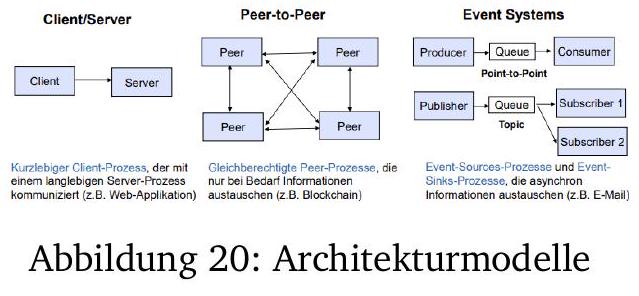
\includegraphics[width=0.9\linewidth]{images/2024_12_29_0d1d7b5551ea1b4b41bdg-18}
\end{concept}

\begin{KR}{Entwurf verteilter Systeme}\\
\textbf{1. Systemanalyse}
\begin{itemize}
    \item Anforderungen identifizieren
    \item Verteilungsaspekte analysieren
    \item Konsistenzanforderungen definieren
\end{itemize}

\textbf{2. Architekturentscheidungen}
\begin{itemize}
    \item Architekturstil wählen
    \item Kommunikationsmuster festlegen
    \item Fehlertoleranzstrategie definieren
\end{itemize}

\textbf{3. Technologieauswahl}
\begin{itemize}
    \item Middleware evaluieren
    \item Protokolle bestimmen
    \item Werkzeuge auswählen
\end{itemize}
\end{KR}

\begin{concept}{Middleware-Technologien}\\
Gängige Technologien für verteilte Systeme:
\begin{itemize}
    \item \textbf{Message Broker:} 
    \begin{itemize}
        \item Apache Kafka
        \item RabbitMQ
    \end{itemize}
    \item \textbf{RPC Frameworks:}
    \begin{itemize}
        \item gRPC
        \item CORBA
    \end{itemize}
    \item \textbf{Web Services:}
    \begin{itemize}
        \item RESTful APIs
        \item GraphQL
    \end{itemize}
\end{itemize}
\end{concept}



\begin{KR}{Typische Fehlerquellen}\\
\textbf{1. Netzwerkfehler}
\begin{itemize}
    \item Verbindungsabbrüche
    \item Timeouts
    \item Partitionierung
\end{itemize}

\textbf{2. Konsistenzprobleme}
\begin{itemize}
    \item Race Conditions
    \item Veraltete Daten
    \item Lost Updates
\end{itemize}

\textbf{3. Skalierungsprobleme}
\begin{itemize}
    \item Lastverteilung
    \item Resource-Management
    \item Bottlenecks
\end{itemize}

\textbf{Lösungsstrategien:}
\begin{itemize}
    \item Circuit Breaker Pattern
    \item Retry mit Exponential Backoff
    \item Idempotente Operationen
    \item Optimistic Locking
\end{itemize}
\end{KR}

	\subsection{Common Pitfalls und Best Practices}

\begin{concept}{Common Pitfalls in JPA Implementation}
\textbf{N+1 Problem:}
\begin{itemize}
    \item \textbf{Symptom:} Für jedes Objekt wird eine zusätzliche Query ausgeführt
    \item \textbf{Lösung:} Join Fetch oder Eager Loading strategisch einsetzen
\end{itemize}

\textbf{LazyInitializationException:}
\begin{itemize}
    \item \textbf{Symptom:} Zugriff auf lazy geladene Referenz außerhalb der Session
    \item \textbf{Lösung:} Transaktionen korrekt abgrenzen
\end{itemize}

\textbf{Bidirektionale Beziehungen:}
\begin{itemize}
    \item \textbf{Symptom:} Inkonsistente Objektzustände
    \item \textbf{Lösung:} Helper-Methoden für Beziehungspflege
\end{itemize}
\end{concept}

\begin{KR}{Best Practices für Persistenz}
\textbf{1. Architektur-Ebene}
\begin{itemize}
    \item Repository für Datenzugriff
    \item Service für Geschäftslogik
    \item DTO für Datentransfer
\end{itemize}

\textbf{2. Entity Design}
\begin{itemize}
    \item Immutable wenn möglich
    \item Bean Validation nutzen
    \item Geschäftsregeln in Entity-Klassen
\end{itemize}

\textbf{3. Performance}
\begin{itemize}
    \item Caching Strategien
    \item Batch Processing
    \item Query Optimierung
\end{itemize}
\end{KR}

\subsection{Parent-Child Beziehungen}

\begin{concept}{Parent-Child Mapping}
\textbf{Implementationsaspekte:}
\begin{itemize}
    \item Cascade-Typen definieren
    \item Bidirektionale Navigation
    \item Lazy Loading konfigurieren
    \item Orphan Removal festlegen
\end{itemize}

\textbf{JPA Annotationen:}
\begin{itemize}
    \item @OneToMany / @ManyToOne
    \item @JoinColumn
    \item mappedBy Parameter
    \item fetch = FetchType.LAZY/EAGER
\end{itemize}
\end{concept}

\subsection{Repository Pattern}

\begin{concept}{Spring Data Repository}
\textbf{Vorteile:}
\begin{itemize}
    \item Standardisierte CRUD-Operationen
    \item Query-Methoden aus Methodennamen
    \item Paginierung und Sortierung
    \item Einfache Integration mit Spring
\end{itemize}

\textbf{Repository Hierarchie:}
\begin{itemize}
    \item Repository (Marker Interface)
    \item CrudRepository (Basis CRUD)
    \item PagingAndSortingRepository
    \item JpaRepository (JPA-spezifisch)
\end{itemize}
\end{concept}

\begin{KR}{Repository Design}
\textbf{1. Interface Definition}
\begin{itemize}
    \item Domänenspezifische Methoden
    \item Query-Methoden
    \item Custom Implementations
\end{itemize}

\textbf{2. Query Methoden}
\begin{itemize}
    \item Methodennamen-Konventionen
    \item @Query Annotation
    \item Native Queries
\end{itemize}

\textbf{3. Transaktionshandling}
\begin{itemize}
    \item @Transactional Annotation
    \item Isolation Level
    \item Propagation Rules
\end{itemize}
\end{KR}

\subsection{Performance Optimierung}

\begin{KR}{Optimierungsstrategien}
\textbf{1. Fetch-Strategien}
\begin{itemize}
    \item Lazy Loading als Default
    \item Joins für häufig benötigte Daten
    \item EntityGraphs für komplexe Szenarien
\end{itemize}

\textbf{2. Caching}
\begin{itemize}
    \item First-Level Cache (Session)
    \item Second-Level Cache
    \item Query Cache
\end{itemize}

\textbf{3. Batch-Verarbeitung}
\begin{itemize}
    \item Batch Inserts/Updates
    \item JDBC Batch Size
    \item Pagination für große Datensätze
\end{itemize}
\end{KR}

%todo: Add examples for:
% - Handling parent-child relationships
% - Repository implementation with Spring Data
% - Performance optimization scenarios
% - Common pitfall solutions

\begin{concept}{Transaktionsmanagement}
\textbf{ACID-Eigenschaften:}
\begin{itemize}
    \item Atomicity (Atomarität)
    \item Consistency (Konsistenz)
    \item Isolation (Isolation)
    \item Durability (Dauerhaftigkeit)
\end{itemize}

\textbf{Isolation Levels:}
\begin{itemize}
    \item READ\_UNCOMMITTED
    \item READ\_COMMITTED
    \item REPEATABLE\_READ
    \item SERIALIZABLE
\end{itemize}
\end{concept}
	\section{Framework Design}

\begin{concept}{Framework Grundlagen}\\
Ein Framework ist ein Programmiergerüst mit folgenden Eigenschaften:
\begin{itemize}
    \item Bietet wiederverwendbare Funktionalität
    \item Definiert Erweiterungs- und Anpassungspunkte
    \item Verwendet Design Patterns
    \item Enthält keinen applikationsspezifischen Code
    \item Gibt Rahmen für anwendungsspezifischen Code vor
    \item Klassen arbeiten eng zusammen (vs. reine Bibliothek)
\end{itemize}
\end{concept}

\begin{definition}{Framework Entwicklung}\\
Die Entwicklung eines Frameworks erfordert:
\begin{itemize}
    \item Höhere Zuverlässigkeit als normale Software
    \item Tiefergehende Analyse der Erweiterungspunkte
    \item Hoher Architektur- und Designaufwand
    \item Sorgfältige Planung der Schnittstellen
\end{itemize}
\end{definition}

\begin{remark}{Kritische Betrachtung}\\
Herausforderungen beim Framework-Einsatz:
\begin{itemize}
    \item Frameworks tendieren zu wachsender Funktionalität
    \item Gefahr von inkonsistentem Design
    \item Funktionale Überschneidungen möglich
    \item Hoher Einarbeitungsaufwand
    \item Schwierige "Scheidung" nach Integration
    \item Trade-off zwischen Abhängigkeit und Nutzen
\end{itemize}
\end{remark}

\subsection{Design Patterns in Frameworks}

\begin{concept}{Abstract Factory}\\
\textbf{Problem:} Erzeugung verschiedener, zusammengehörender Objekte ohne Kenntnis konkreter Klassen\\
\textbf{Lösung:}
\begin{itemize}
    \item AbstractFactory-Interface definieren
    \item Pro Produkt eine create-Methode
    \item Konkrete Factories implementieren Interface
\end{itemize}
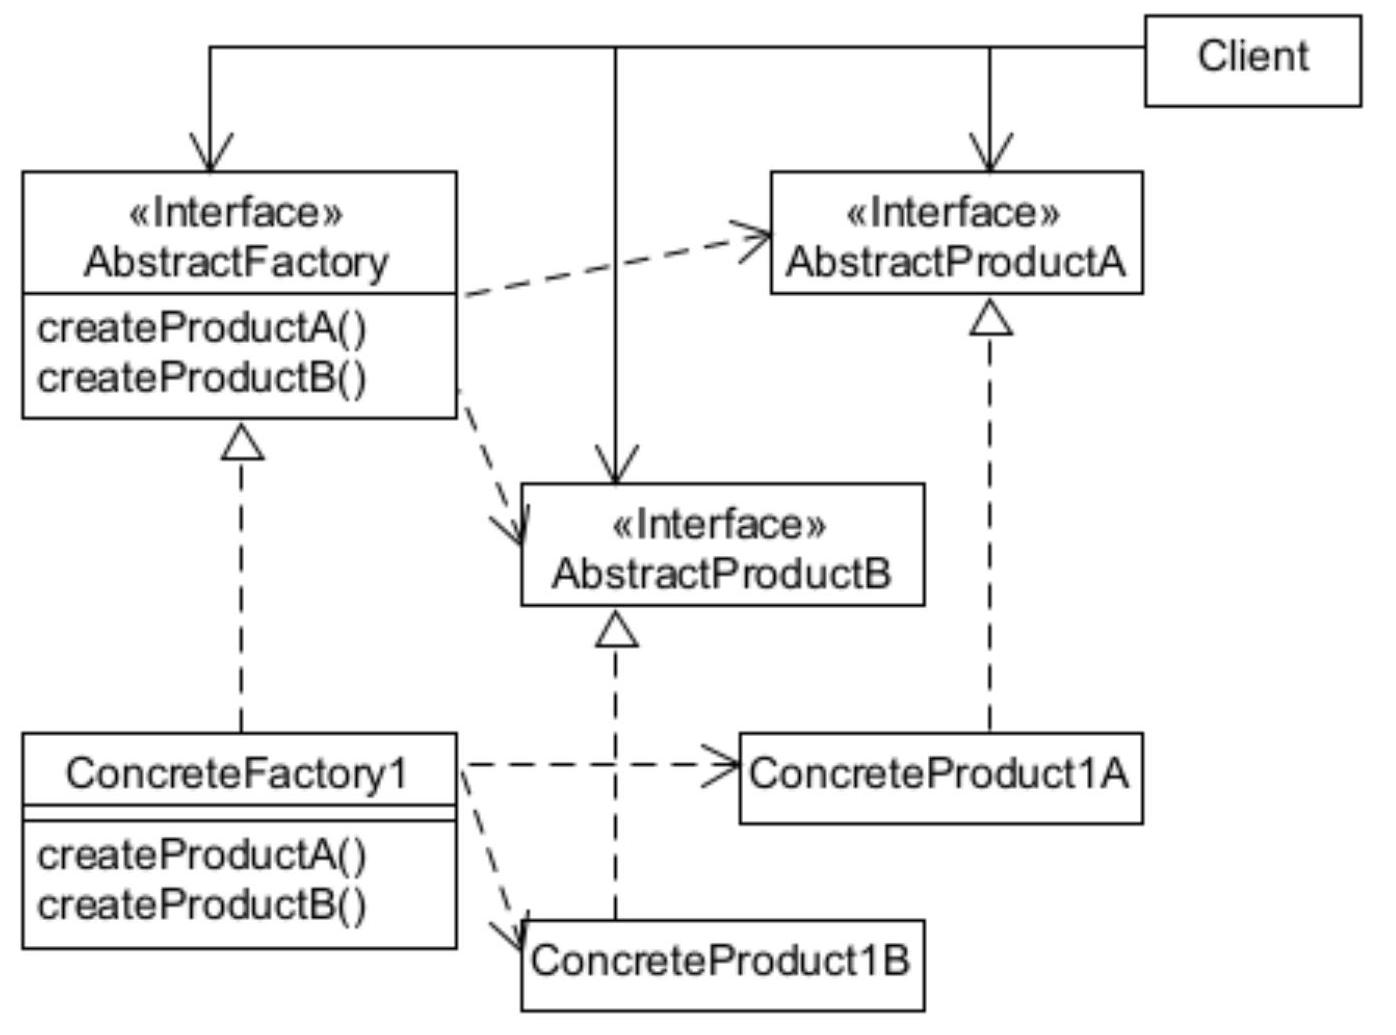
\includegraphics[width=0.8\linewidth]{images/2025_01_02_73d93f10fa91ab6123dcg-13}
\end{concept}

\begin{example}{Abstract Factory: POS Terminal}
\begin{lstlisting}[language=Java, style=base]
public interface IJavaPOSDevicesFactory {
    CashDrawer getNewCashDrawer();
    CoinDispenser getNewCoinDispenser();
    // weitere Methoden
}

public class IBMJavaPOSDevicesFactory 
        implements IJavaPOSDevicesFactory {
    public CashDrawer getNewCashDrawer() {
        return new com.ibm.pos.jpos.CashDrawer();
    }
    // weitere Implementierungen
}
\end{lstlisting}
\end{example}

\begin{concept}{Factory Method}\\
\textbf{Problem:} Flexible Objekterzeugung in wiederverwendbarer Klasse\\
\textbf{Lösung:}
\begin{itemize}
    \item Abstrakte Factory-Methode in Creator-Klasse
    \item Konkrete Subklassen überschreiben Methode
    \item Parallele Vererbungshierarchien
\end{itemize}
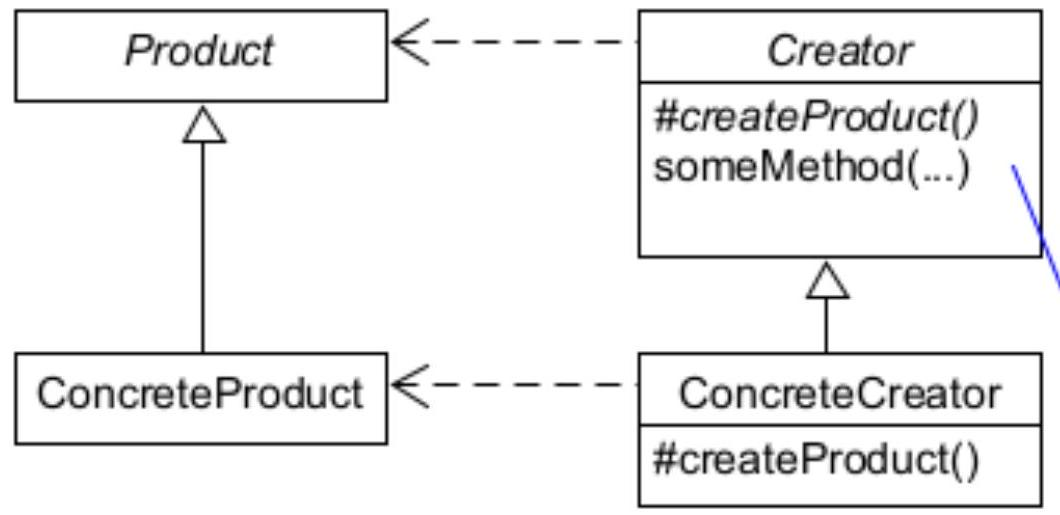
\includegraphics[width=0.8\linewidth]{images/2025_01_02_73d93f10fa91ab6123dcg-16}
\end{concept}

\begin{concept}{Command}\\
\textbf{Problem:} Aktionen für späteren Gebrauch speichern und verwalten\\
\textbf{Lösung:}
\begin{itemize}
    \item Command-Interface definieren
    \item Konkrete Commands implementieren
    \item Parameter für Ausführung speichern
    \item Optional: Undo-Funktionalität
\end{itemize}
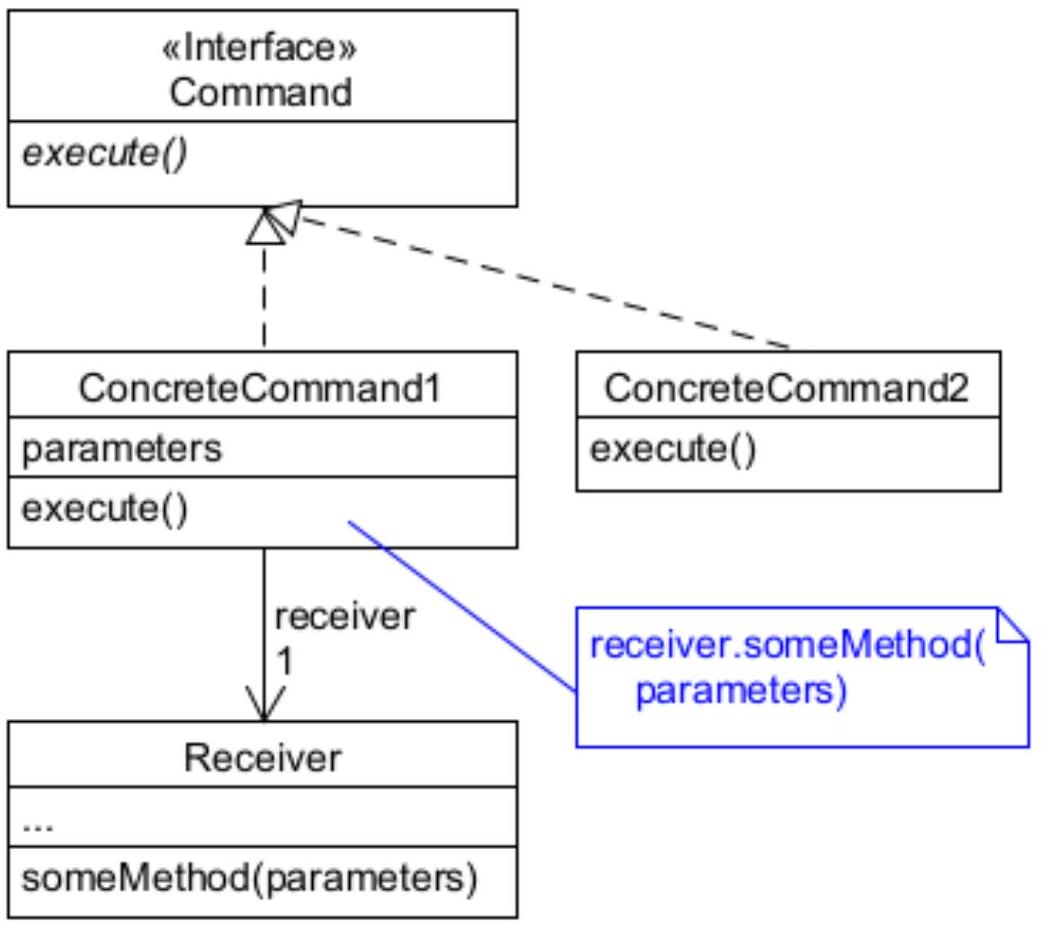
\includegraphics[width=0.8\linewidth]{images/2025_01_02_73d93f10fa91ab6123dcg-19}
\end{concept}

\begin{example}{Command: Persistenz}
\begin{lstlisting}[language=Java, style=base]
public interface ICommand {
    void execute();
    void undo();
}

public class DBUpdateCommand implements ICommand {
    private PersistentObject object;
    
    public void execute() {
        // Update in Datenbank
    }
    
    public void undo() {
        // Aenderung rueckgaengig machen
    }
}
\end{lstlisting}
\end{example}

\begin{concept}{Template Method}\\
\textbf{Problem:} Algorithmus mit anpassbaren Teilschritten\\
\textbf{Lösung:}
\begin{itemize}
    \item Template Method in abstrakter Klasse
    \item Hook-Methoden für variable Teile
    \item Hollywood Principle: "Don't call us, we'll call you"
\end{itemize}
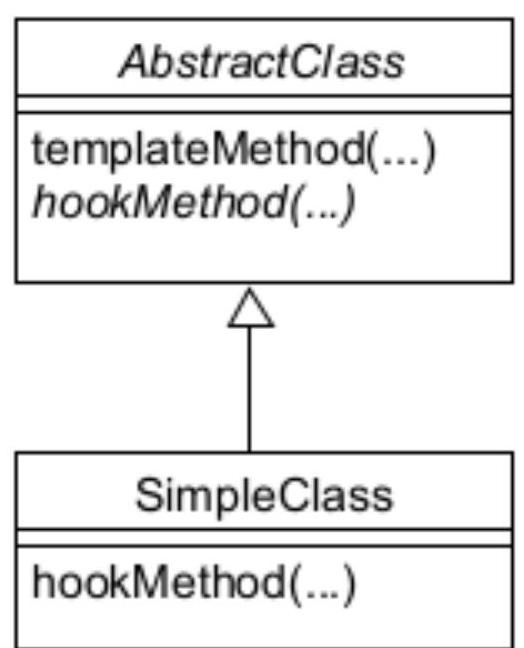
\includegraphics[width=0.8\linewidth]{images/2025_01_02_73d93f10fa91ab6123dcg-22}
\end{concept}

\begin{example}{Template Method: GUI Framework}
\begin{lstlisting}[language=Java, style=base]
public abstract class GUIComponent {
    // Template Method
    public final void update() {
        clearBackground();
        repaint(); // Hook Method
    }
    
    protected abstract void repaint();
}

public class MyButton extends GUIComponent {
    protected void repaint() {
        // Button-spezifische Implementation
    }
}
\end{lstlisting}
\end{example}

\subsection{Moderne Framework Patterns}

\begin{concept}{Annotation-basierte Konfiguration}\\
Moderne Frameworks nutzen Annotationen für:
\begin{itemize}
    \item Dependency Injection
    \item Konfiguration
    \item Interface-Implementation
    \item Funktionalitätserweiterung
\end{itemize}
\end{concept}

\begin{KR}{Framework Integration}
\begin{enumerate}
    \item \textbf{Convention over Configuration}
    \begin{itemize}
        \item Namenskonventionen einhalten
        \item Standard-Verhalten nutzen
        \item Nur Ausnahmen konfigurieren
    \end{itemize}
    
    \item \textbf{Dependency Injection}
    \begin{itemize}
        \item Abhängigkeiten deklarieren
        \item Framework übernimmt Injection
        \item Constructor- oder Setter-Injection
    \end{itemize}
    
    \item \textbf{Interface-basierte Entwicklung}
    \begin{itemize}
        \item Interfaces definieren
        \item Framework generiert Implementation
        \item Methodennamen als Spezifikation
    \end{itemize}
\end{enumerate}
\end{KR}

\begin{example}{Spring Data Repository}
\begin{lstlisting}[language=Java, style=base]
@Repository
public interface UserRepository 
        extends JpaRepository<User, Long> {
    // Methode wird automatisch implementiert
    List<User> findByLastNameOrderByFirstNameAsc(
        String lastName);
    
    // SQL-Query via Annotation
    @Query("SELECT u FROM User u WHERE u.active = true")
    List<User> findActiveUsers();
}
\end{lstlisting}
\end{example}

\begin{remark}
Annotation-basierte Frameworks bieten:
\begin{itemize}
    \item Geringere Kopplung zur Framework-API
    \item Deklarativen Programmierstil
    \item Reduzierte Boilerplate-Code
    \item Kann aber zu längeren Startzeiten führen
\end{itemize}
\end{remark}
	\section{wrapup}

\section*{Angewendeter iterativ-inkrementeller Softwareentwicklungsprozess in SWEN1/PM3}
\begin{itemize}
  \item Der Softwareentwicklungsprozess wurde so angepasst (engl. tailoring), dass die wesentlichen Artefakte in einem Softwareprojekt im Kontext eingeführt werden können.
  \item Die Software wird in Iterationen entwickelt (2 Wochen Rhythmus).
  \item Jede Iteration hat ein Ziel und wird nach Abschluss reviewed.
  \item Es gibt drei Meilensteine, die im Projektverlauf ein besonderes Ereignis darstellen bzw. den Abschluss einer Phase: Projektskizze (M1), Lösungsarchitektur (M2) und Beta-Release (M3)
  \item In jeder Iteration werden Anforderungen, Analyse \& Design, Implementation und Testing gemacht (Software entsteht in Inkrementen).
  \item Der angewendete Softwareentwicklungsprozess und das Projektmanagement eines iterativ-inkrementellen Projektes wird in PM3 noch detaillierter erklärt.
\end{itemize}

\section*{Wesentliche Resultate bzw. Artefakte}
\begin{itemize}
  \item Anforderungsanalyse
  \item Funktionale Anforderungen mit Use Cases
  \item Qualitätsanforderungen und Randbedingungen
  \item Domänenmodell
  \item Design
  \item Softwarearchitektur
  \item Use Case Realisierung (statische und dynamische Modelle)
  \item Implementation
  \item Quellcode (inkl. Javadoc)
  \item Testing
  \item Unit-Tests\\
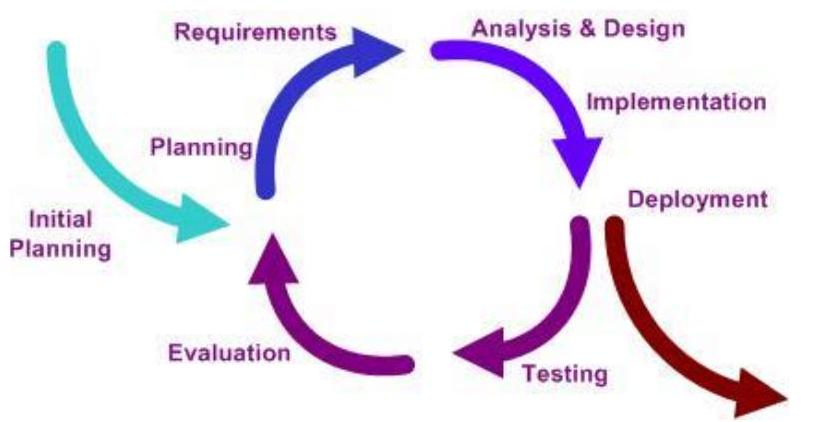
\includegraphics[max width=\textwidth, center]{2025_01_02_6eafa38dd4ae10c9a392g-09}
  \item Integrations- und Systemtests
\end{itemize}

\section*{Modellierung und Modelle mit der UML}

\includegraphics[max width=\textwidth, center]{2025_01_02_6eafa38dd4ae10c9a392g-10}\\
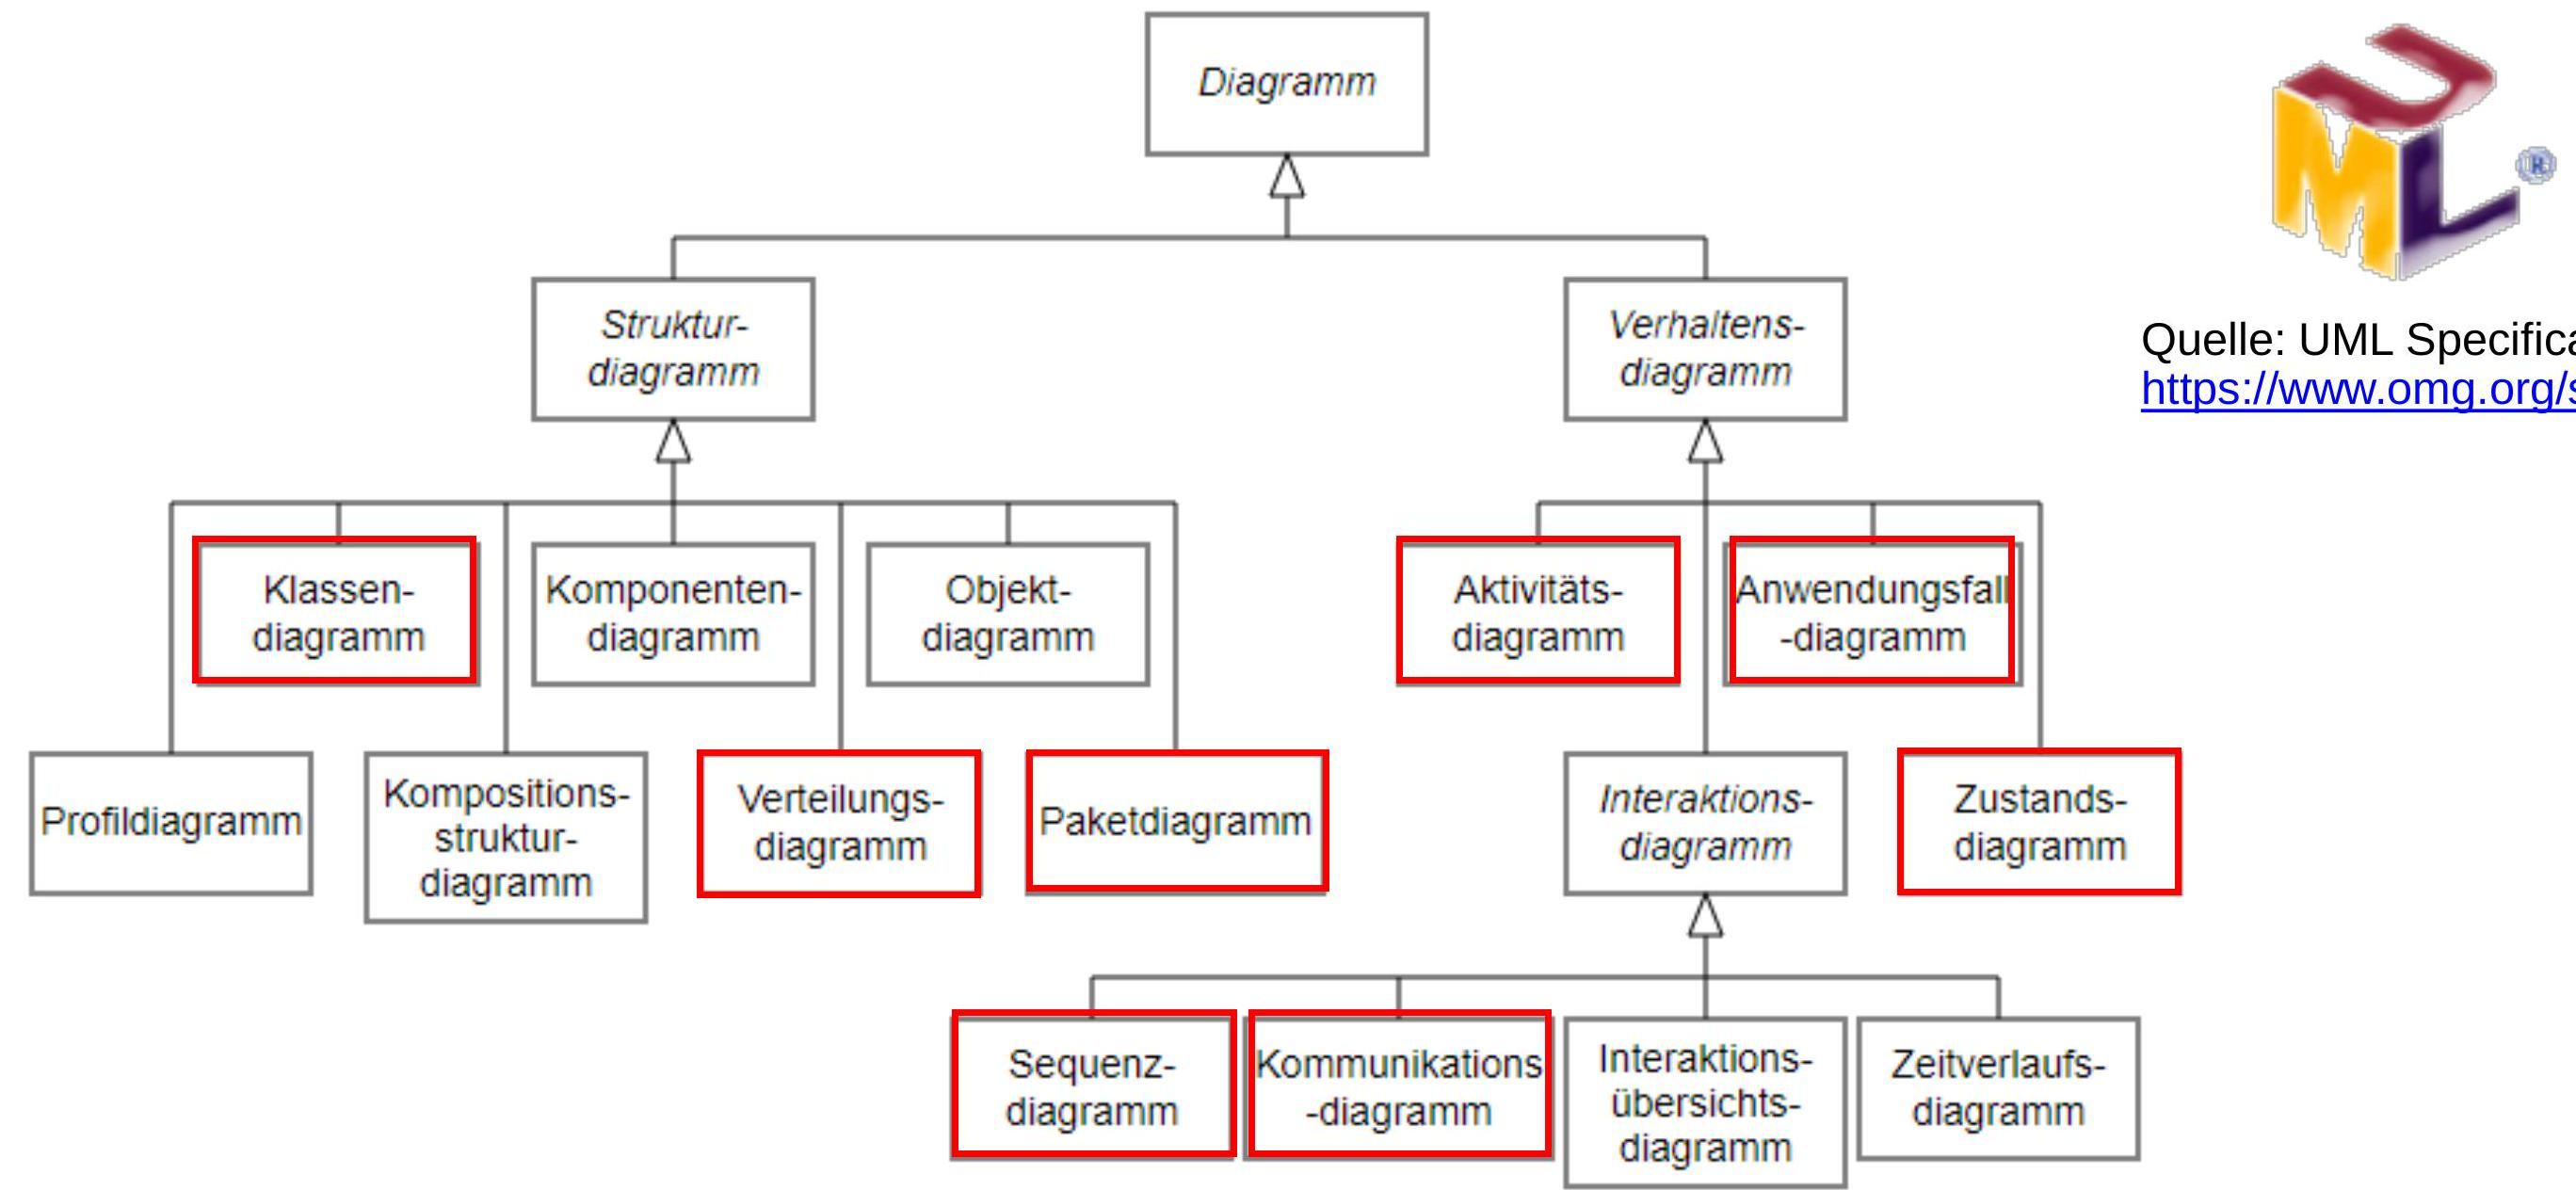
\includegraphics[max width=\textwidth, center]{2025_01_02_6eafa38dd4ae10c9a392g-10(1)}

Quelle: UML Specification, \href{https://www.omg.org/spec/UML/}{https://www.omg.org/spec/UML/}\\
$\square$ für die Modellierung in SWEN1 relevant

\section*{Gebrauch der UML (nach Martin Fowler)}
\section*{- UML as a Sketch}
\begin{itemize}
  \item Informelle und unvollständige Diagramme (z.T. von Hand gezeichnet), um schwierige Teile des Problems oder der Lösung zu verstehen und zu kommunizieren
  \item Die agile Community bevorzugt diese Anwendungsart von UML
  \item UML as a Blueprint
  \item Relativ detaillierte Analyse und Design-Diagramme für Code-Generierung oder um existierenden Code besser zu verstehen
  \item Klassische UML-Tools für ein Forward- und Reverse-Engineering (Roundtrip)
  \item UML as a Programming Language
  \item Komplete, ausführbare Spezifikation eines Software-Systems in UML
  \item MDA-Tools zur Modellierung und Generierung
\end{itemize}

\section*{Überblick Anforderungen \& Analyse}
\begin{itemize}
  \item User Research (Personas und Szenarien, Contextual Inquiry)
  \item Sketching und Protoyping
  \item Ableiten und Modellieren von Use Cases (dt. Anwendungsfälle)
  \item Detaillierung der Use Case (UML-Use-Case-Diagramm, Use-CaseSpezifikationen, UI-Sketching
  \item Qualitätsanforderungen und Randbedingungen erheben und festhalten.
  \item Modellierung der Fachlichkeit und Begriffe des Anwenders in einem Domänenmodell (konzeptuelles UML-Klassendiagramm)
  \item Bei der objektorientierten Analyse (OOA) liegt die Betonung darauf, die Objekte - oder Konzepte in dem Problembereich zu finden und zu beschreiben!
\end{itemize}

\section*{Überblick Design}
\begin{itemize}
  \item Design und Modellierung einer für die Problemstellung geeigneten Softwarearchitektur (UML-Paketdiagramm, UML-Verteilungsdiagramm)
  \item Use-Case-Realisierung und Klassendesign mit Verantwortlichkeiten (UML-Klassendiagramm, UML-Sequenzdiagramm, UMLKommunikationsdiagramm, UML-Zustandsdiagramm, UML-\\
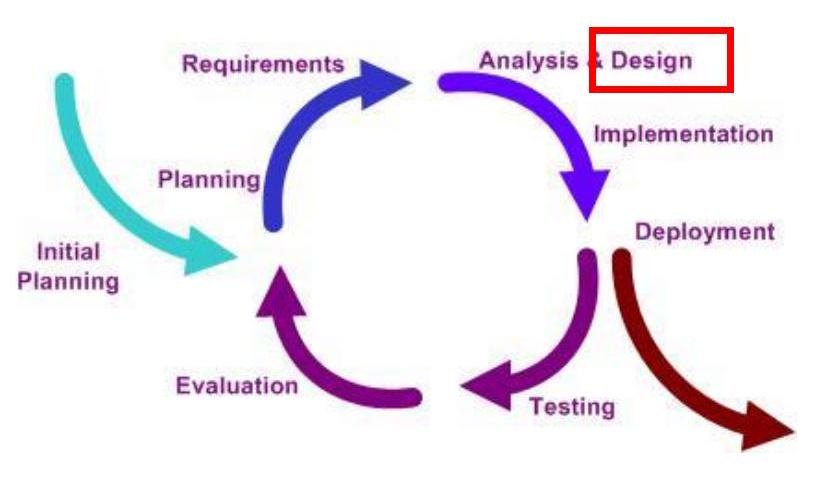
\includegraphics[max width=\textwidth]{2025_01_02_6eafa38dd4ae10c9a392g-13} Aktivitätsdiagramm)
  \item Entwurf mit bewährten Design Patterns
  \item Beim objektorientierten Design (OOD) liegt die Betonung darauf, geeignete Softwareobjekte und ihr Zusammenwirken (engl. collaboration) zu definieren, um die Anforderungen zu erfüllen!
\end{itemize}

\section*{Überblick Implementation}
\begin{itemize}
  \item Umsetzung des Designs in Code der entsprechenden (objektorientierten) Programmiersprache
  \item Verwendung von geeigneten Algorithmen und Datenstrukturen zur Implementierung des Designs
  \item Code Smells sofort bei deren Aufdeckung verbessern (Refactoring)\\
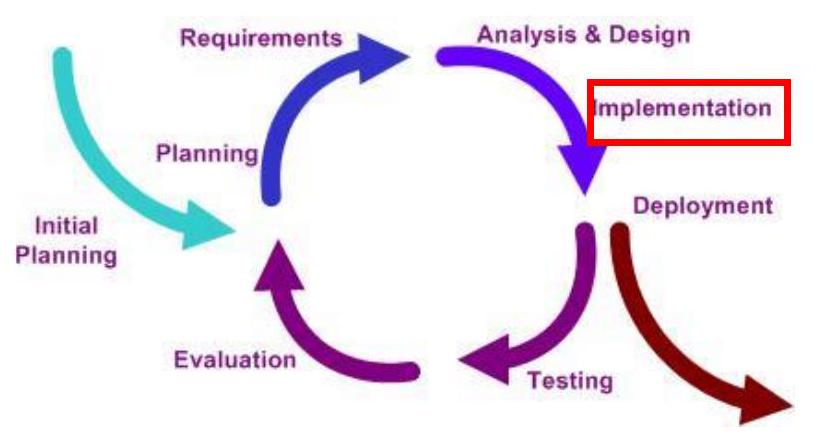
\includegraphics[max width=\textwidth, center]{2025_01_02_6eafa38dd4ae10c9a392g-14}
  \item Laufende Dokumentation des Quellcodes (nach Clean CodePrinzipien)
\end{itemize}

\section*{Überblick Testing}
\begin{itemize}
  \item Laufendes Design und Implementierung von Unit-Tests
  \item Planung, Design und Durchführung von weiteren Tests auf den Teststufen Integration und System je nach Problemstellung
  \item Dokumentation des Testkonzepts und der Tests\\
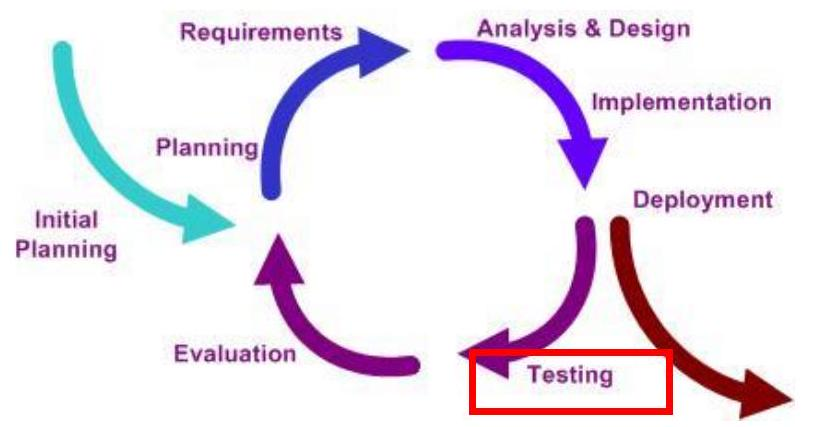
\includegraphics[max width=\textwidth, center]{2025_01_02_6eafa38dd4ae10c9a392g-15}
\end{itemize}
	\raggedcolumns
	\pagebreak
	\section{Additional Examples}

\subsection{Rechnerarithmetik}

\begin{example2}{Werteberechnung ausführlich} 
Gegeben sei die Maschinenzahl zur Basis $B=2$:
$$x = \underbrace{0.1101}_{\text{n=4}} \cdot \underbrace{2^{101}_2}_{\text{l=3}}$$

\textbf{1. Normalisierung prüfen:}
\begin{itemize}
    \item $m_1 = 1 \neq 0$ $\rightarrow$ normalisiert
\end{itemize}

\textbf{2. Exponent berechnen:}
\begin{align*}
\hat{e} &= 1 \cdot 2^2 + 0 \cdot 2^1 + 1 \cdot 2^0 \\
&= 4 + 0 + 1 = 5
\end{align*}

\textbf{3. Wert berechnen:}
\begin{align*}
\hat{\omega} &= 1 \cdot 2^{5-1} + 1 \cdot 2^{5-2} + 0 \cdot 2^{5-3} + 1 \cdot 2^{5-4} \\
&= 1 \cdot 2^4 + 1 \cdot 2^3 + 0 \cdot 2^2 + 1 \cdot 2^1 \\
&= 16 + 8 + 0 + 2 \\
&= 26
\end{align*}

Also ist $x = 26$
\end{example2}

\begin{example2}{Weitere Beispiele}
\begin{enumerate}
    \item Basis 10: $0.3141 \cdot 10^2$
    \begin{itemize}
        \item Normalisiert, da $m_1 = 3 \neq 0$
        \item $\hat{e} = 2$
        \item $\hat{\omega} = 3 \cdot 10^1 + 1 \cdot 10^0 + 4 \cdot 10^{-1} + 1 \cdot 10^{-2} = 31.41$
    \end{itemize}
    
    \item Basis 16 (hex): $0.A5F \cdot 16^3$
    \begin{itemize}
        \item Normalisiert, da $m_1 = A = 10 \neq 0$
        \item $\hat{e} = 3$
        \item $\hat{\omega} = 10 \cdot 16^2 + 5 \cdot 16^1 + 15 \cdot 16^0 = 2655$
    \end{itemize}
\end{enumerate}
\end{example2}

\begin{example2}{Werteberechnung} Berechnung einer Zahl zur Basis B=2:
\begin{minipage}{0.45\textwidth}
    $$\underbrace{0.1011}_{\text{n=4}} \cdot \underbrace{2^{3}}_{\text{l=1}}$$
\end{minipage}
\begin{minipage}[t]{0.5\textwidth}
    1. Exponent: $\hat{e} = 3$ \\ 
    2. Wert: $\hat{\omega} = 1\cdot2^2 + 0\cdot2^1 + 1\cdot2^0 + 1\cdot2^{-1}$ \\
    $= 4 + 0 + 1 + 0.5 = 5.5$
\end{minipage}
\end{example2}

\raggedcolumns


\subsection{Numerische Lösung von Nullstellenproblemen}

\begin{example2}{Fixpunktiteration} Nullstellen von $p(x)=x^3-x+0.3$\\
    %TODO: check if this is correct and/or relevant - either correct or replace with better example
Fixpunktgleichung: $x_{n+1} = F(x_n) = x_n^3 + 0.3$
\begin{enumerate}
    \item $F'(x) = 3x^2$ steigt monoton
    \item Für $I=[0,0.5]$: $F(0)=0.3 > 0$, $F(0.5)=0.425 < 0.5$
    \item $\alpha = \max_{x \in [0,0.5]} |3x^2| = 0.75 < 1$
    \item Konvergenz für Startwerte in $[0,0.5]$ gesichert
\end{enumerate}
\end{example2}



\begin{example2}{Newton-Verfahren} Berechnung von $\sqrt[3]{2}$
Nullstellenproblem: $f(x)=x^3-2$
\vspace{1mm}\\
\begin{minipage}[t]{0.65\textwidth}
    \vspace{-3mm}
    Ableitung: $f'(x)=3x^2$, Startwert $x_0=1$
    \begin{enumerate}
        \item $x_1 = 1 - \frac{1^3-2}{3 \cdot 1^2} = 1.333333$
        \item $x_2 = 1.333333 - \frac{1.333333^3-2}{3 \cdot 1.333333^2} = 1.259921$
        \item $x_3 = 1.259921 - \frac{1.259921^3-2}{3 \cdot 1.259921^2} = 1.259921$
    \end{enumerate}
\end{minipage}
\begin{minipage}[t]{0.3\textwidth}
    Quadratische Konvergenz sichtbar durch schnelle Annäherung an $\sqrt[3]{2} \approx 1.259921$
\end{minipage}
\end{example2}

\begin{example2}{Newton vs Sekanten}
Bestimmen Sie $\sqrt{2}$ mit beiden Verfahren.

\paragraph{Newton-Verfahren:} $f(x) = x^2-2$
\begin{itemize}
    \item $f'(x) = 2x$
    \item $x_0 = 1.5$
    \item $x_1 = 1.5 - \frac{1.5^2-2}{2\cdot1.5} = 1.4167$
    \item $x_2 = 1.4167 - \frac{1.4167^2-2}{2\cdot1.4167} = 1.4142$
\end{itemize}

\paragraph{Sekantenverfahren:}
\begin{itemize}
    \item $x_0 = 1$, $x_1 = 2$
    \item $x_2 = x_1 - \frac{x_1-x_0}{f(x_1)-f(x_0)}f(x_1) = 1.5$
    \item $x_3 = 1.5 - \frac{1.5-2}{1.5^2-2}1.5 = 1.4545$
    \item $x_4 = 1.4545 - \frac{1.4545-1.5}{1.4545^2-2}1.4545 = 1.4143$
\end{itemize}

\paragraph{Vergleich:}
\begin{itemize}
    \item Newton: Schnellere Konvergenz (quadratisch)
    \item Sekanten: Keine Ableitungsberechnung nötig
    \item Beide erreichen $10^{-4}$ Genauigkeit in 4-5 Schritten
\end{itemize}
\end{example2}

\subsection{Numerische Lösung von LGS}

\begin{example2}{Pivotisierung in der Praxis}
Betrachten Sie das System:
$$\begin{psmallmatrix}
0.001 & 1\\
1 & 1
\end{psmallmatrix}
\begin{psmallmatrix}
x_1\\
x_2
\end{psmallmatrix} = 
\begin{psmallmatrix}
1\\
2
\end{psmallmatrix}$$

\paragraph{Ohne Pivotisierung:}
Division durch 0.001 führt zu großen Rundungsfehlern:
$$x_1 \approx 1000 \cdot (1 - x_2)$$

\paragraph{Mit Pivotisierung:}
Nach Zeilenvertauschung:
$$\begin{psmallmatrix}
1 & 1\\
0.001 & 1
\end{psmallmatrix}
\begin{psmallmatrix}
x_1\\
x_2
\end{psmallmatrix} = 
\begin{psmallmatrix}
2\\
1
\end{psmallmatrix}$$
Liefert stabile Lösung: $x_1 = 1$, $x_2 = 1$
\end{example2}

\begin{example2}{Gauss mit Pivotisierung}
Lösen Sie $Ax = b$ mit:
$$A = \begin{pmatrix} 
1 & 2 & 1 \\
2 & 4 & -1 \\
4 & -2 & 1
\end{pmatrix}, \quad b = \begin{pmatrix} 1 \\ 2 \\ 0 \end{pmatrix}$$

\paragraph{Lösung:}
\begin{enumerate}
    \item Erste Spalte: Pivot $a_{31} = 4$ $\rightarrow$ Z1 $\leftrightarrow $ Z3
    $$\begin{pmatrix} 
    4 & -2 & 1 & | & 0 \\
    2 & 4 & -1 & | & 2 \\
    1 & 2 & 1 & | & 1
    \end{pmatrix}$$
    
    \item Eliminationsschritte:
    $$\begin{pmatrix} 
    4 & -2 & 1 & | & 0 \\
    0 & 5 & -1.5 & | & 2 \\
    0 & 2.5 & 0.75 & | & 1
    \end{pmatrix}$$
    $$\begin{pmatrix} 
    4 & -2 & 1 & | & 0 \\
    0 & 5 & -1.5 & | & 2 \\
    0 & 0 & 1.5 & | & 0.2
    \end{pmatrix}$$
    
    \item Rückwärtseinsetzen:
    \begin{align*}
        x_3 &= 0.2/1.5 = \frac{2}{15} \\
        x_2 &= (2 + 1.5 \cdot \frac{2}{15})/5 = 0.5 \\
        x_1 &= (0 + 2 \cdot 0.5 - 1 \cdot \frac{2}{15})/4 = 0.2
    \end{align*}
\end{enumerate}
\end{example2}

\begin{example2}{LR-Zerlegung mit Pivotisierung}
Gegeben sei das System:
$$A = \begin{psmallmatrix}
1 & 2 & 1\\
3 & 8 & 1\\
0 & 4 & 1
\end{psmallmatrix}, \quad b = \begin{psmallmatrix}
2\\
3\\
5
\end{psmallmatrix}$$

\paragraph{1. Erste Spalte}
Max Element in 1. Spalte: $|a_{21}| = 3$, tausche Z1 und Z2:
$$P_1 = \begin{psmallmatrix}
0 & 1 & 0\\
1 & 0 & 0\\
0 & 0 & 1
\end{psmallmatrix}, \quad 
A^{(1)} = \begin{psmallmatrix}
3 & 8 & 1\\
1 & 2 & 1\\
0 & 4 & 1
\end{psmallmatrix}$$

Eliminationsfaktoren: $l_{21} = \frac{1}{3}$, $l_{31} = 0$\\
Nach Elimination:
$$A^{(2)} = \begin{psmallmatrix}
3 & 8 & 1\\
0 & -\frac{2}{3} & \frac{2}{3}\\
0 & 4 & 1
\end{psmallmatrix}$$

\paragraph{2. Zweite Spalte}
Max Element: $|a_{32}| = 4$, tausche Z2 und Z3:
$$P_2 = \begin{psmallmatrix}
1 & 0 & 0\\
0 & 0 & 1\\
0 & 1 & 0
\end{psmallmatrix}$$

Eliminationsfaktor: $l_{32} = -\frac{1}{6}$\\
Nach Elimination:
$$R = \begin{psmallmatrix}
3 & 8 & 1\\
0 & 4 & 1\\
0 & 0 & \frac{5}{6}
\end{psmallmatrix}$$

\paragraph{Endergebnis}
$$P = P_2P_1 = \begin{psmallmatrix}
0 & 1 & 0\\
0 & 0 & 1\\
1 & 0 & 0
\end{psmallmatrix}, \quad
L = \begin{psmallmatrix}
1 & 0 & 0\\
\frac{1}{3} & 1 & 0\\
0 & -\frac{1}{6} & 1
\end{psmallmatrix}$$

\paragraph{Lösung des Systems}
\begin{enumerate}
    \item $Pb = \begin{psmallmatrix} 3\\ 5\\ 2 \end{psmallmatrix}$
    \item $Ly = Pb$: $y = \begin{psmallmatrix} 3\\ 4\\ 1 \end{psmallmatrix}$
    \item $Rx = y$: $x = \begin{psmallmatrix} 1\\ 0\\ \frac{6}{5} \end{psmallmatrix}$
\end{enumerate}
\end{example2}

\begin{KR}{Umgang mit Systemen mit freien Variablen}
\begin{enumerate}
    \item Vorgehensweise
    \begin{itemize}
        \item Matrix auf Stufenform bringen
        \item Freie Variablen identifizieren (Nullspalten)
        \item Basislösung berechnen
        \item Allgemeine Lösung parametrisch aufstellen
    \end{itemize}
    
    \item Interpretation
    \begin{itemize}
        \item Rang der Matrix bestimmen
        \item Lösbarkeit prüfen
        \item Dimension des Lösungsraums bestimmen
        \item Spezielle Lösungen generieren
    \end{itemize}
    
    \item Sonderfälle beachten
    \begin{itemize}
        \item Unlösbare Systeme erkennen
        \item Abhängige Gleichungen identifizieren
        \item Numerische Genauigkeit berücksichtigen
    \end{itemize}
\end{enumerate}
\end{KR}

\begin{example2}{QR-Zerlegung}
Gegeben sei die Matrix:
$$A = \begin{psmallmatrix}
1 & 1\\
1 & 0\\
0 & 1
\end{psmallmatrix}$$

\paragraph{1. Erste Spalte}
$v_1 = \begin{psmallmatrix} 1\\ 1\\ 0 \end{psmallmatrix}$, 
$\|v_1\| = \sqrt{2}$

Householder-Vektor:
$w_1 = v_1 + \sqrt{2}\begin{psmallmatrix} 1\\ 0\\ 0 \end{psmallmatrix} = 
\begin{psmallmatrix} 1+\sqrt{2}\\ 1\\ 0 \end{psmallmatrix}$

Normierung:
$u_1 = \frac{1}{\sqrt{4+2\sqrt{2}}}
\begin{psmallmatrix} 1+\sqrt{2}\\ 1\\ 0 \end{psmallmatrix}$

Erste Householder-Matrix:
$$H_1 = I - 2u_1u_1^T = 
\begin{psmallmatrix}
-\frac{1}{\sqrt{2}} & -\frac{1}{\sqrt{2}} & 0\\
-\frac{1}{\sqrt{2}} & \frac{1}{\sqrt{2}} & 0\\
0 & 0 & 1
\end{psmallmatrix}$$

\paragraph{2. Zweite Spalte}
Nach Anwendung von $H_1$:
$$H_1A = \begin{psmallmatrix}
-\sqrt{2} & -\frac{1}{\sqrt{2}}\\
0 & \frac{1}{\sqrt{2}}\\
0 & 1
\end{psmallmatrix}$$

Untervektor für zweite Transformation:
$v_2 = \begin{psmallmatrix} \frac{1}{\sqrt{2}}\\ 1 \end{psmallmatrix}$

Analog zur ersten Transformation erhält man:
$$H_2 = \begin{psmallmatrix}
1 & 0 & 0\\
0 & -\frac{1}{\sqrt{5}} & -\frac{2}{\sqrt{5}}\\
0 & -\frac{2}{\sqrt{5}} & \frac{1}{\sqrt{5}}
\end{psmallmatrix}$$

\paragraph{Endergebnis}
$$Q = H_1^TH_2^T = \begin{psmallmatrix}
\frac{1}{\sqrt{2}} & \frac{1}{\sqrt{2}} & 0\\
\frac{1}{\sqrt{2}} & -\frac{1}{\sqrt{2}} & 0\\
0 & 0 & 1
\end{psmallmatrix}$$

$$R = H_2H_1A = \begin{psmallmatrix}
\sqrt{2} & 1\\
0 & \sqrt{2}\\
0 & 0
\end{psmallmatrix}$$

\paragraph{Verifikation}
\begin{itemize}
    \item $Q^TQ = QQ^T = I$ (Orthogonalität)
    \item $QR = A$ (bis auf Rundungsfehler)
    \item R ist obere Dreiecksmatrix
\end{itemize}
\end{example2}

\begin{example2}{Iterative Verfahren}{Vergleich Jacobi und Gauss-Seidel}
System:
$$\begin{psmallmatrix}
4 & -1 & 0\\
-1 & 4 & -1\\
0 & -1 & 4
\end{psmallmatrix}x = \begin{psmallmatrix}
1\\
5\\
0
\end{psmallmatrix}$$

\begin{center}
\begin{tabular}{c|cc|cc}
k & \multicolumn{2}{c|}{Jacobi} & \multicolumn{2}{c}{Gauss-Seidel}\\
\hline
0 & $(0,0,0)^T$ & & $(0,0,0)^T$ &\\
1 & $(0.25,1.25,0)^T$ & 1.25 & $(0.25,1.31,0.08)^T$ & 1.31\\
2 & $(0.31,1.31,0.31)^T$ & 0.31 & $(0.33,1.33,0.33)^T$ & 0.02\\
3 & $(0.33,1.33,0.33)^T$ & 0.02 & $(0.33,1.33,0.33)^T$ & 0.00
\end{tabular}
\end{center}
\end{example2}




\subsection{Eigenvektoren und Eigenwerte}

\begin{example2}{Darstellungsformen}
Gegeben: $z = 3 - 11i$ in Normalform
$$r = \sqrt{3^2 + 11^2} = \sqrt{130}, \quad \varphi = \arcsin(\frac{11}{\sqrt{130}}) = 1.3 \text{rad} = 74.74^{\circ}$$
\textbf{Trigonometrische Form:} $z = \sqrt{130}(\cos(1.3) + i\sin(1.3))$
\vspace{2mm}\\
\textbf{Exponentialform:} $z = \sqrt{130}e^{i\cdot 1.3}$
\end{example2}

\begin{example2}{Eigenwertberechnung}
%TODO: check if this is correct and/or relevant - either correct or replace with better example
$A = \begin{psmallmatrix} 1 & 0 & 0\\ 2 & 3 & 0\\ 0 & 1 & 2\end{psmallmatrix}$
\begin{enumerate}
    \item Da $A$ eine Dreiecksmatrix ist, sind die Diagonalelemente die \\
    Eigenwerte:
    $\lambda_1 = 1, \lambda_2 = 3, \lambda_3 = 2$
    \item $\det(A) = \lambda_1\cdot\lambda_2\cdot\lambda_3 = 6$
    \item $\operatorname{tr}(A) = \lambda_1 + \lambda_2 + \lambda_3 = 6$
    \item Spektrum: $\sigma(A) = \{1,2,3\}$
\end{enumerate}
\end{example2}

\begin{example2}{Von-Mises-Iteration}
Berechne größten Eigenwert der Matrix:
\vspace{2mm}\\
$A = \begin{psmallmatrix}
4 & -1 & 1\\
-1 & 3 & -2\\
1 & -2 & 3
\end{psmallmatrix}$, $\quad$
Startvektor: $v^{(0)} = \begin{psmallmatrix}1\\ 0\\ 0\end{psmallmatrix}$

\begin{center}
\begin{tabular}{c|c|c}
k & $v^{(k)}$ & $\lambda^{(k)}$ \\\hline
0 & $(1, 0, 0)^T$ & -\\
1 & $(0.970, -0.213, 0.119)^T$ & 4.000\\
2 & $(0.957, -0.239, 0.164)^T$ & 4.827\\
3 & $(0.953, -0.244, 0.178)^T$ & 4.953\\
4 & $(0.952, -0.245, 0.182)^T$ & 4.989
\end{tabular}
\end{center}

Konvergenz gegen $\lambda_1 \approx 5$ \\ Eigenvektor $v \approx (0.952, -0.245, 0.182)^T$
\end{example2}

\begin{example2}{Von-Mises-Iteration}
Bestimmen Sie den betragsmäßig größten Eigenwert von:
$$A = \begin{psmallmatrix}
3 & 1 \\
1 & 3
\end{psmallmatrix}$$

\paragraph{Lösung:}
\begin{enumerate}
    \item Start mit $v^{(0)} = \frac{1}{\sqrt{2}}\begin{psmallmatrix} 1 \\ 1 \end{psmallmatrix}$
    
    \item Erste Iteration:
    \begin{itemize}
        \item $w^{(0)} = \begin{psmallmatrix} 4 \\ 4 \end{psmallmatrix}$
        \item $v^{(1)} = \frac{1}{\sqrt{2}}\begin{psmallmatrix} 1 \\ 1 \end{psmallmatrix}$
        \item $\lambda^{(1)} = 4$
    \end{itemize}
    
    \item Ergebnis:
    \begin{itemize}
        \item Eigenvektor bereits gefunden
        \item Eigenwert $\lambda = 4$ ist korrekt
    \end{itemize}
\end{enumerate}
\end{example2}

\begin{example2}{QR-Verfahren}
Matrix:
$$A = \begin{psmallmatrix}
2 & -1 & 1\\
-1 & 3 & 0\\
1 & 0 & 1
\end{psmallmatrix}$$

\paragraph{QR-Iteration:}
\begin{enumerate}
    \item $A_0 = A$
    \item Nach erster Iteration:
    $$A_1 = \begin{psmallmatrix}
    3.21 & -0.83 & 0.62\\
    -0.83 & 2.13 & 0.41\\
    0.62 & 0.41 & 0.66
    \end{psmallmatrix}$$
    \item Nach 5 Iterationen:
    $$A_5 \approx \begin{psmallmatrix}
    4 & 0 & 0\\
    0 & 1 & 0\\
    0 & 0 & 1
    \end{psmallmatrix}$$
\end{enumerate}

Die Diagonalelemente von $A_5$ sind die Eigenwerte: $\lambda_1 = 4, \lambda_2 = 1, \lambda_3 = 1$
\end{example2}
	\raggedcolumns
\end{multicols}
\end{document}
